%% Do not edit unless you really know what you are doing.
\documentclass[english]{beamer}
\usepackage[T1]{fontenc}
\usepackage[latin9]{inputenc}
\setcounter{secnumdepth}{3}
\setcounter{tocdepth}{3}
\usepackage{amsfonts}
\usepackage{amssymb}
\usepackage{amsmath}
\usepackage{amsthm}
\usepackage{mathtools}
\usepackage{verbatim}
\usepackage{graphicx}
\usepackage{epstopdf}
\usepackage{amstext}
\usepackage{beamerthemesplit}
\usepackage{float}
\usepackage{tipa}
\usepackage{fancyhdr}
\usepackage{rotating}
\usepackage{natbib}
\usepackage{multicol}


\makeatletter
%%%%%%%%%%%%%%%%%%%%%%%%%%%%%% Textclass specific LaTeX commands.
 % this default might be overridden by plain title style
 \newcommand\makebeamertitle{\frame{\maketitle}}%
 \AtBeginDocument{
   \let\origtableofcontents=\tableofcontents
   \def\tableofcontents{\@ifnextchar[{\origtableofcontents}{\gobbletableofcontents}]}
   \def\gobbletableofcontents#1{\origtableofcontents}
 }

%%%%%%%%%%%%%%%%%%%%%%%%%%%%%% User specified LaTeX commands.


%\usepackage{beamerthemeshadow}

% Setting theme for presentation slides
\usetheme{Madrid} \usecolortheme{seahorse}
%\newcommand*\oldmacro{}
%\let\oldmacro\insertshorttitle % save previous definition
%\renewcommand*\insertshorttitle{
%\oldmacro \hfill  \leftskip=.2cm
%  \insertframenumber\,/\,\inserttotalframenumber}
\setbeamertemplate{footline}
{
  \leavevmode%
  \hbox{%
  \begin{beamercolorbox}[wd=.333333\paperwidth,ht=2.25ex,dp=1ex,center]{author in head/foot}%
    \usebeamerfont{author in head/foot}\insertsection
  \end{beamercolorbox}%
  \begin{beamercolorbox}[wd=.333333\paperwidth,ht=2.25ex,dp=1ex,center]{title in head/foot}%
    \usebeamerfont{title in head/foot}\insertsubsection
  \end{beamercolorbox}%
  \begin{beamercolorbox}[wd=.333333\paperwidth,ht=2.25ex,dp=1ex,right]{date in head/foot}%
    \usebeamerfont{date in head/foot}\insertshortdate{}\hspace*{2em}
    \insertframenumber{} / \inserttotalframenumber\hspace*{2ex} 
  \end{beamercolorbox}}%
  \vskip0pt%
}

\makeatother

\newcommand{\EEp}[1]{\mathbb{E}\left[#1\right]}
\newcommand{\R}{\mathbb{R}}
\newcommand{\norm}[1]{\|#1\|}
\newcommand{\snorm}[1]{\left\|#1\right\|} % scaling norm

\newcommand{\bi}{\begin{itemize}[<+->]}
\newcommand{\ei}{\end{itemize}}
\newcommand{\bc}{\begin{center}}
\newcommand{\ec}{\end{center}}
\newcommand{\eps}{\epsilon}
\newcommand{\nologo}{\setbeamertemplate{logo}{}} 
\newcommand{\ds}{$\diamondsuit$}

\begin{document}

\title{Deterministic Independent Component Analysis (ICA)}


\author{Ruitong Huang\hspace{4mm} Andr\'{a}s Gy\"{o}rgy \hspace{4mm}
 Csaba Szepesv\'ari}


\institute{University of Alberta}


\date{July 8, 2015 }
%\logo{{\centering 
\includegraphics[width=5cm]{UA-CMPSCI-COLOUR.png} \hspace{0.5cm} 
\includegraphics[width=3cm]{logo.jpg}}\hspace{0.2cm}}

\titlegraphic{
\includegraphics[height=8mm]{UA-CMPSCI-COLOUR} \hspace{150pt} 
\includegraphics[height=10mm]{logo} \hspace{5pt}}
\date{\today}

\makebeamertitle

\begin{frame}
\frametitle{Outline}
\tableofcontents 
\end{frame}


\section{Introduction}
\subsection{What is ICA, really? A little bit of philosophy for machine learning theorists}
\frame{ \frametitle{What is Independent Component Analysis (ICA)?}

\bc
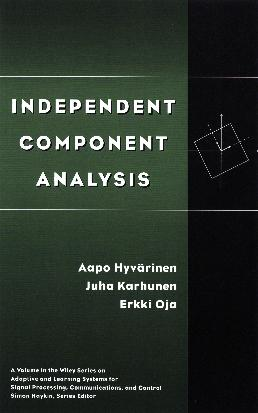
\includegraphics[height=\textheight]{ICABookCover}
\ec

%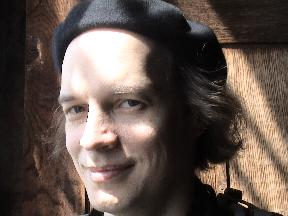
\includegraphics{Aapo}
%\begin{block}{}
%Independent component analysis (ICA) is a statistical and computational technique for revealing hidden factors that underlie sets of random variables, measurements, or signals.
%\end{block}
}

\frame{
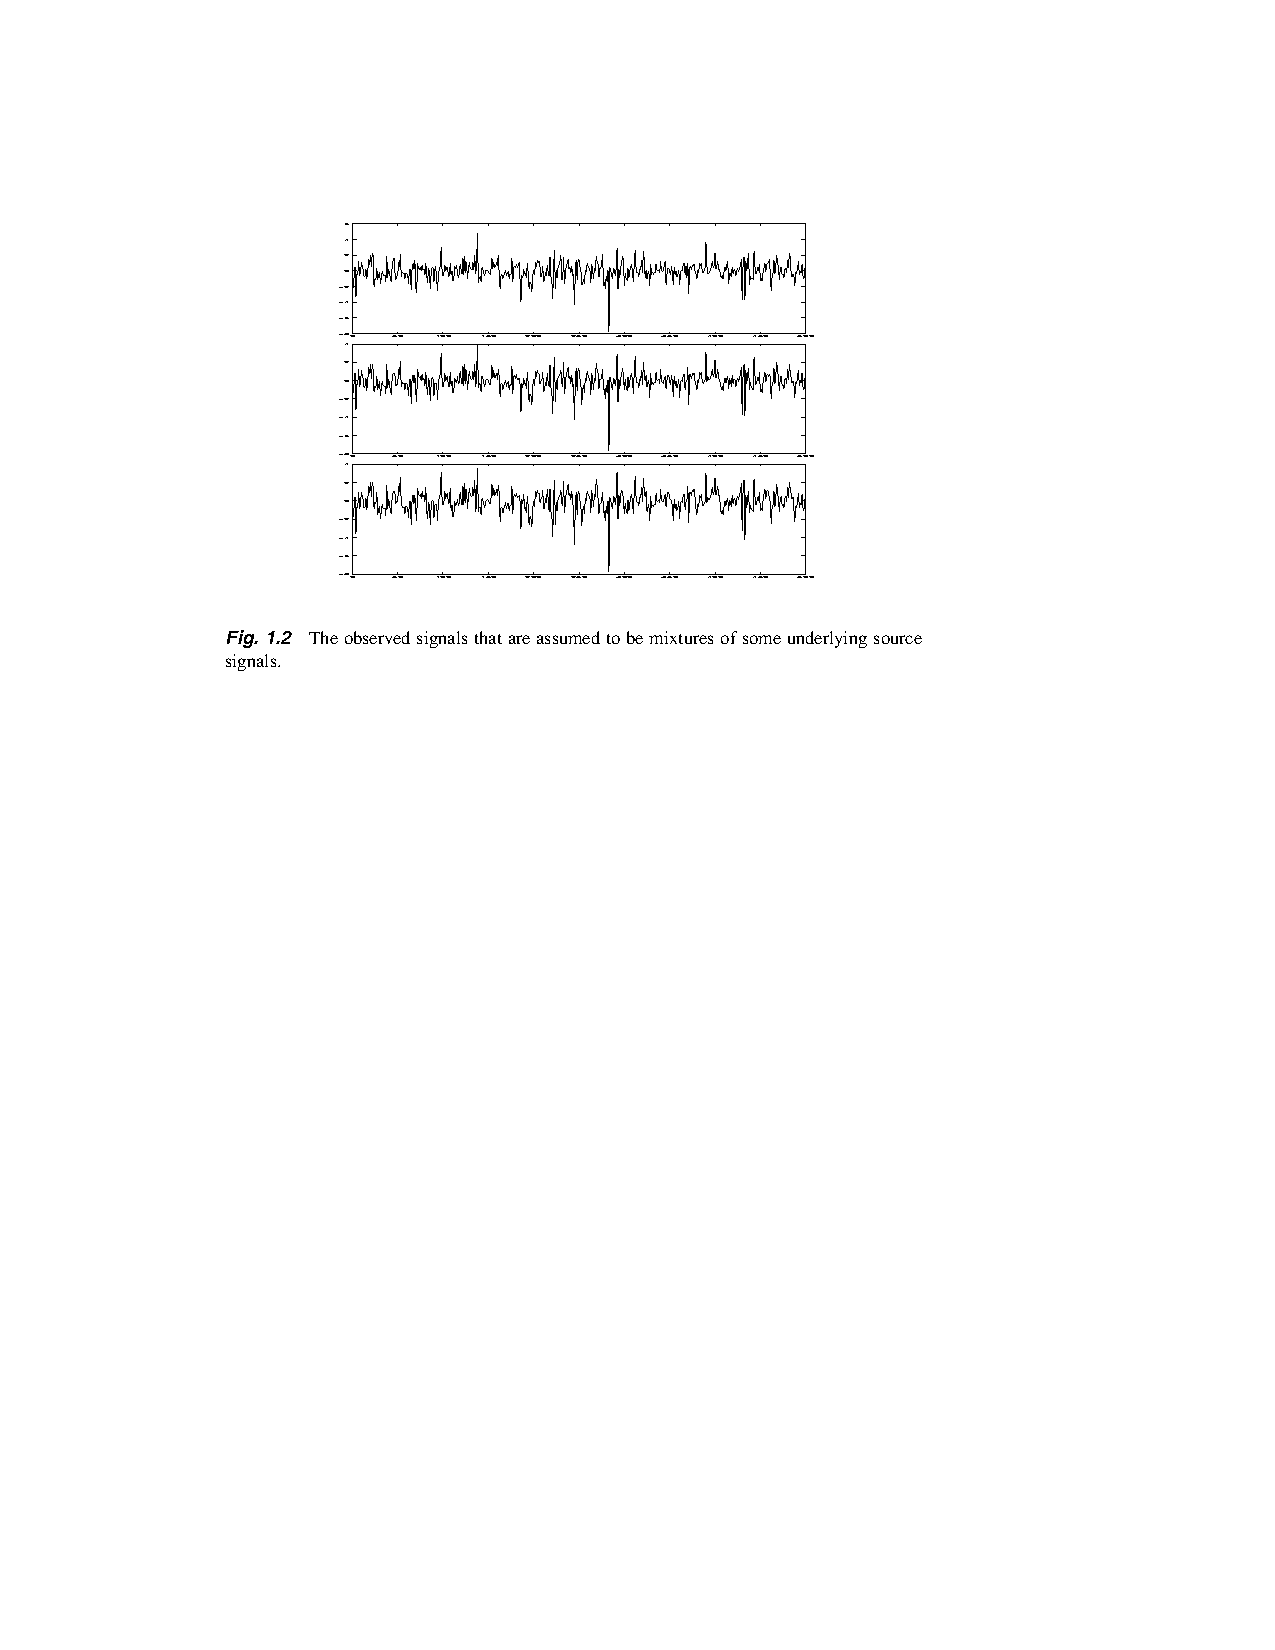
\includegraphics{ICABOOK2001_ObservedSignals}
}

\frame{
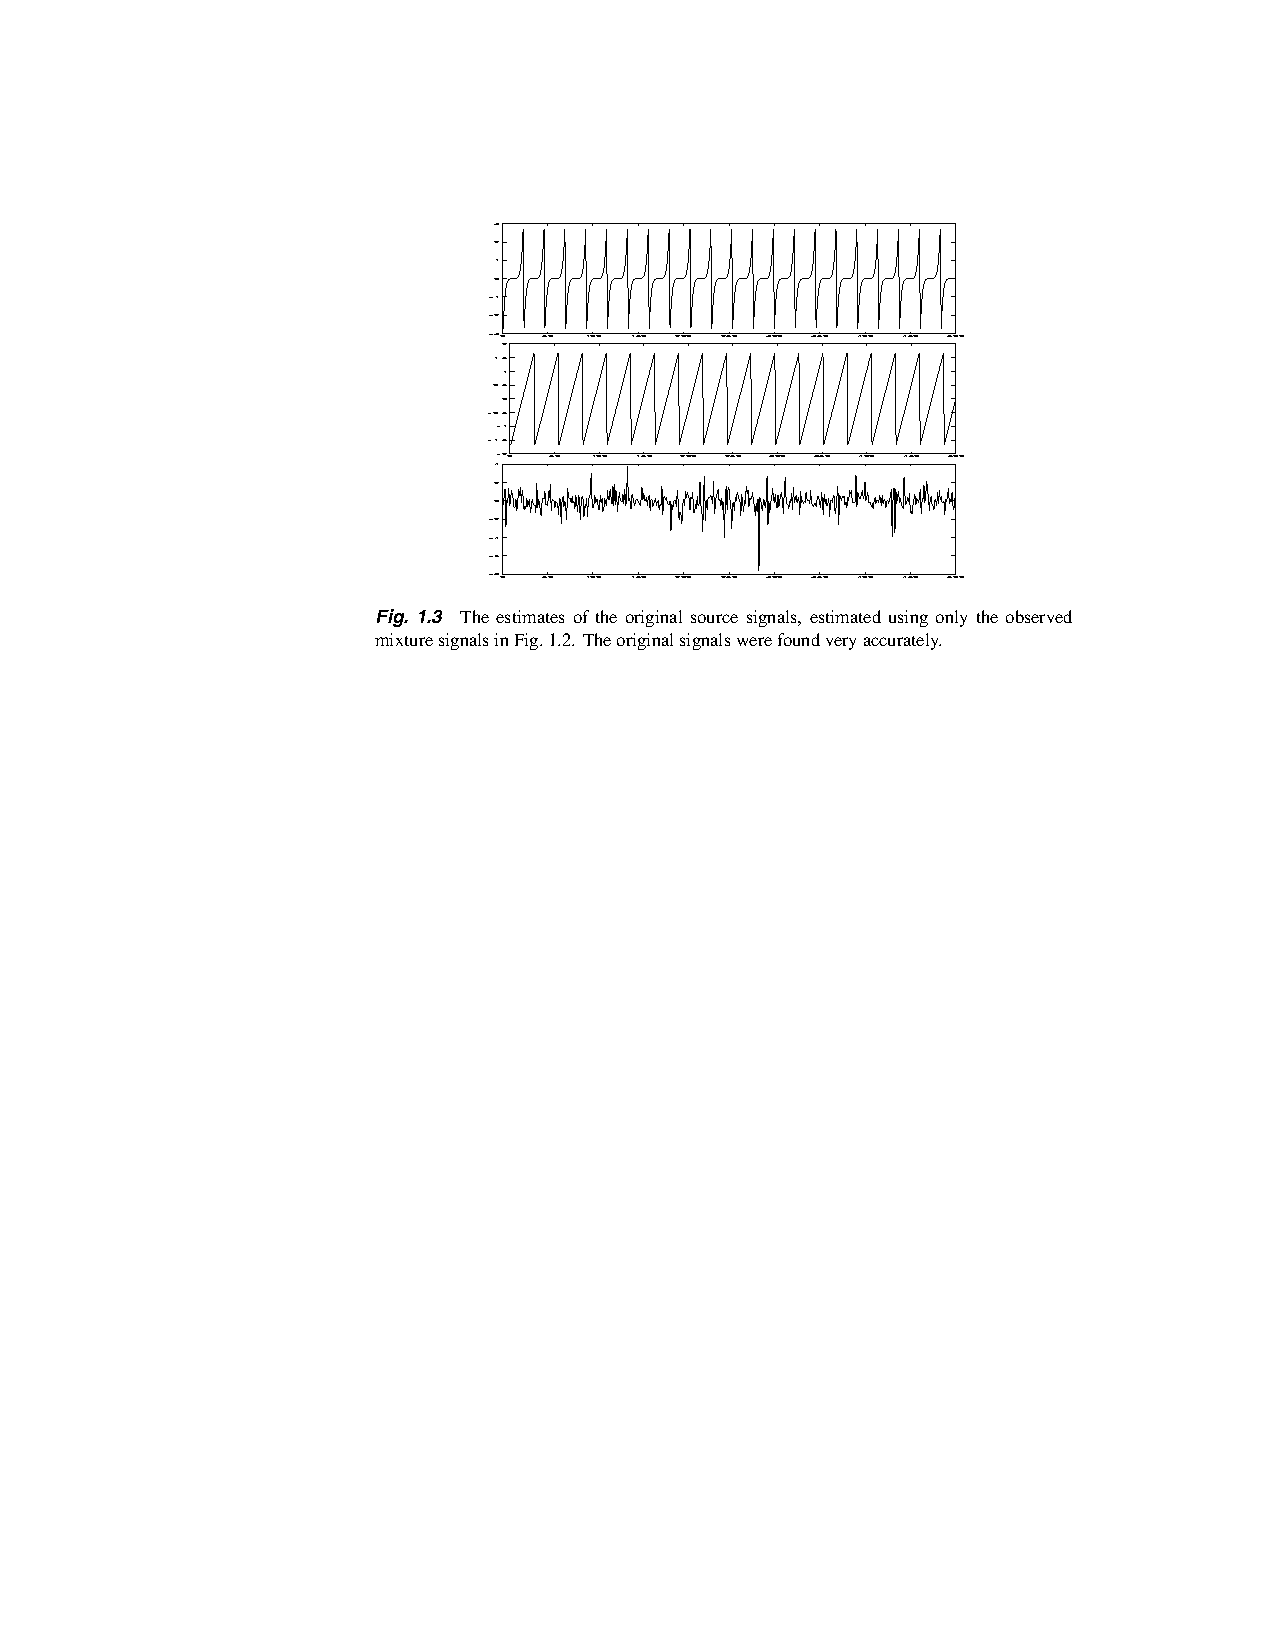
\includegraphics{ICABOOK2001_ReconstructedSignals}
}

\frame{
{
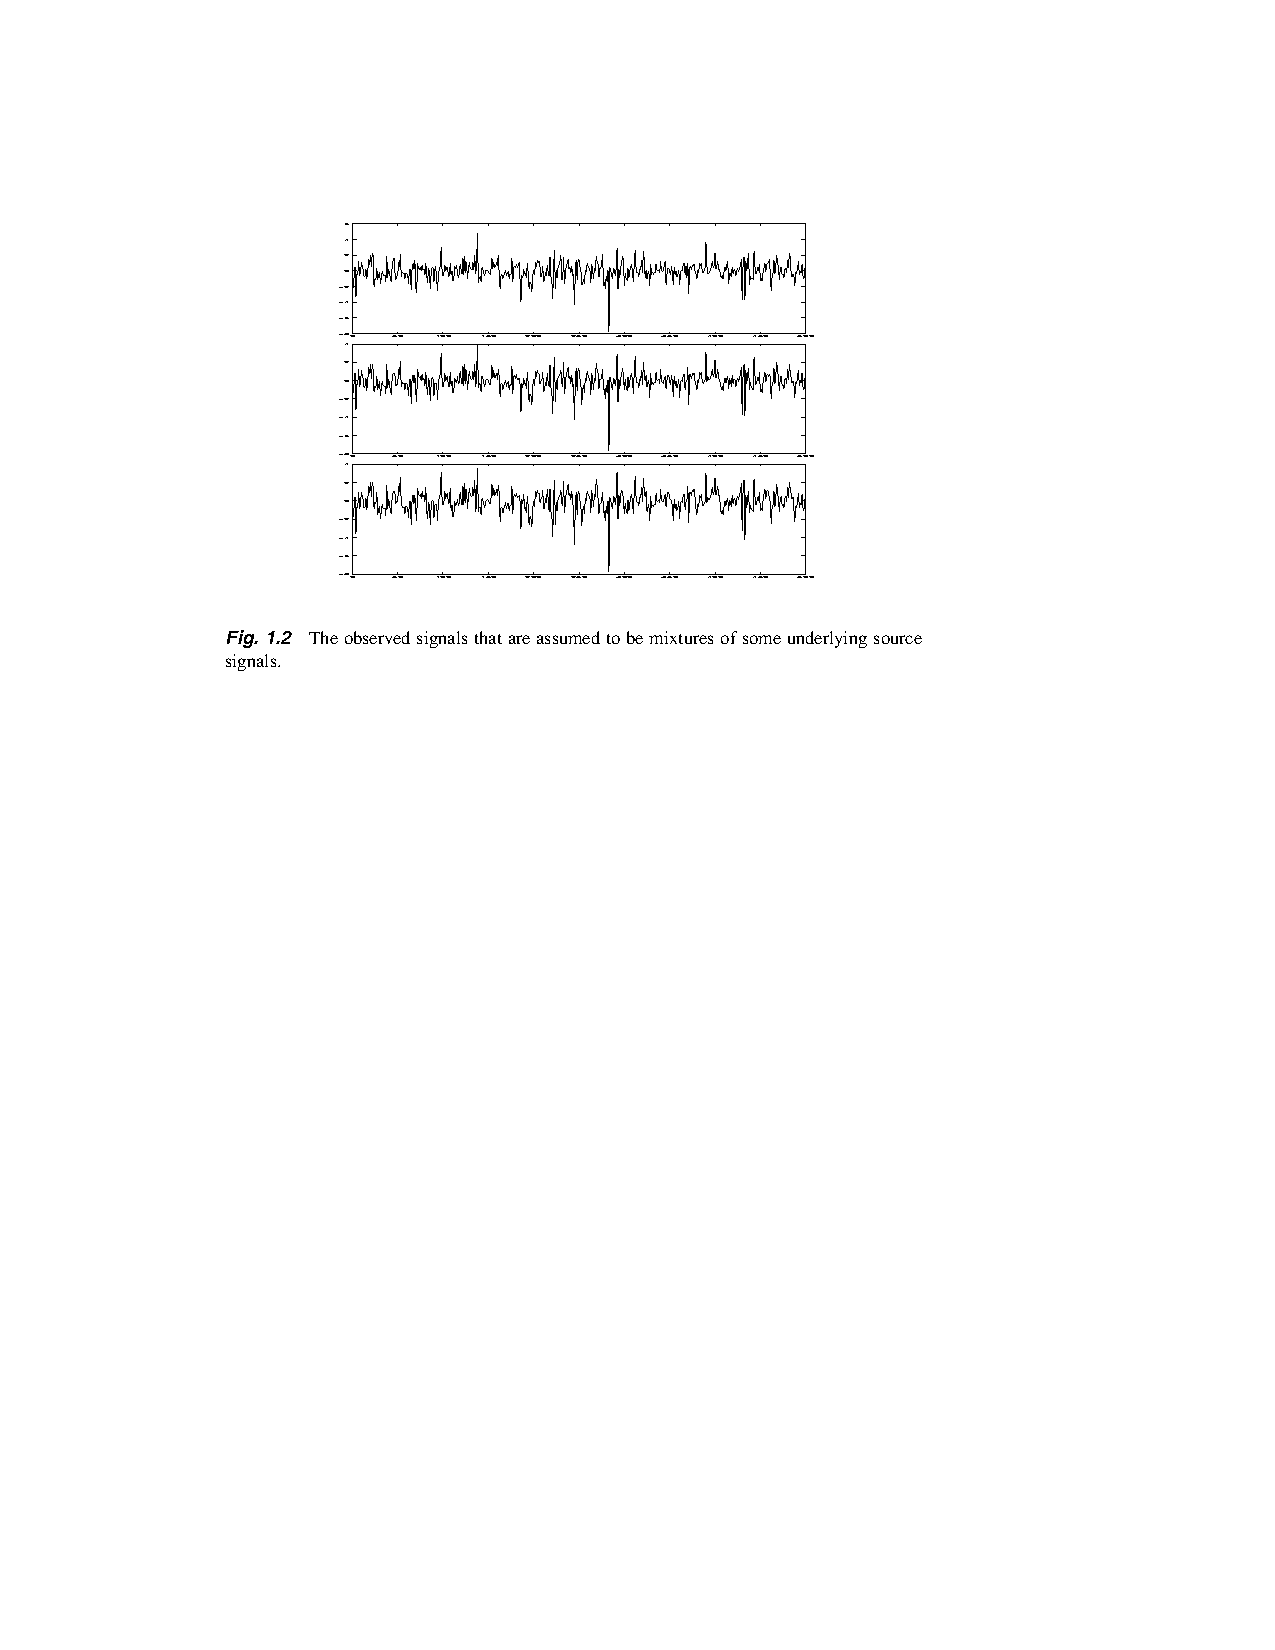
\includegraphics[width=0.3\textwidth]{ICABOOK2001_ObservedSignals}
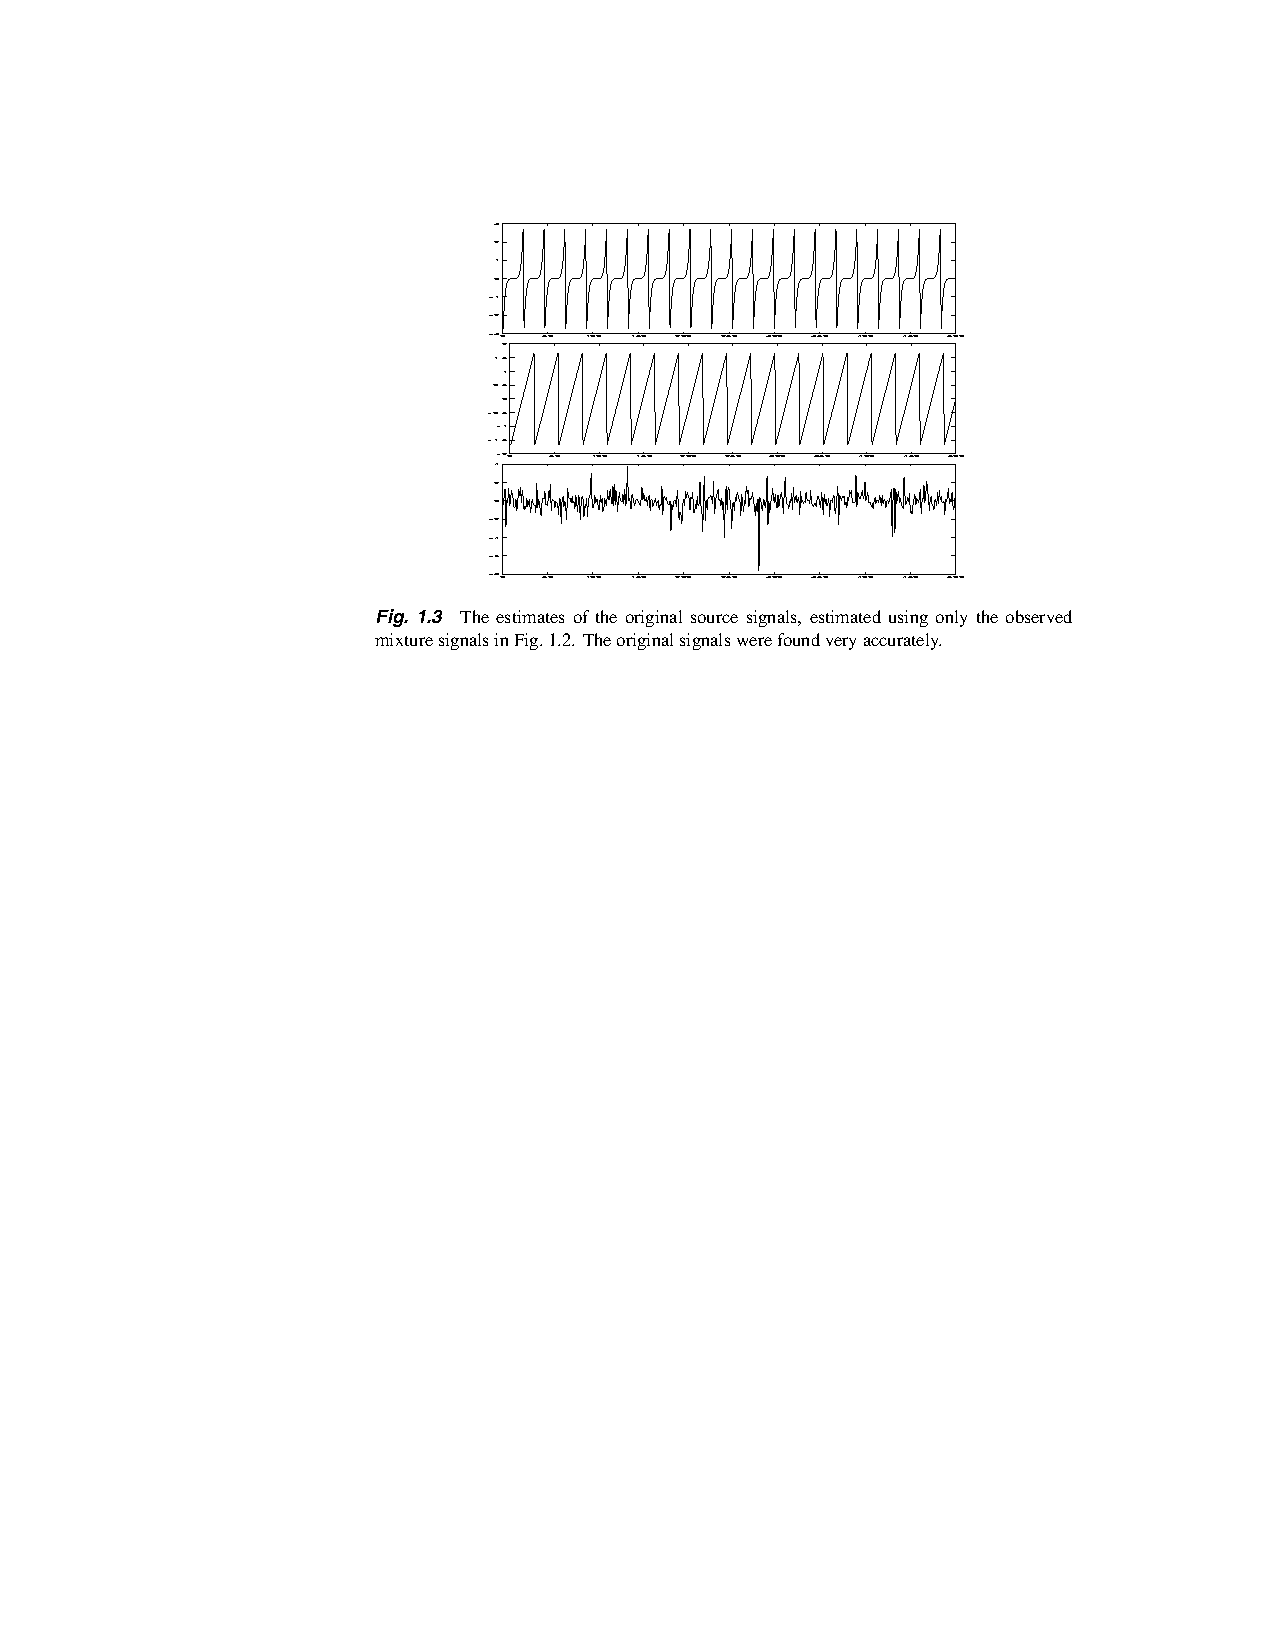
\includegraphics[width=0.3\textwidth]{ICABOOK2001_ReconstructedSignals}
}
%\vspace*{-0.5in}
\begin{quotation}
\uncover<+->{%
``Using just this information on the \alert{statistical independence}, we can in fact estimate the coefficient matrix $W$ for the signals in Fig. 1.2. 
}
\uncover<+->{%
What we obtain are the source signals in Fig. 1.3. (These signals were estimated by the FastICA algorithm that we shall meet in several chapters of this book.)}
\uncover<+->{%
We see that from a data set that seemed to be just noise, we were able to estimate the original source signals, using an algorithm that used the information on the \alert{independence only}.
}
\uncover<+->{%
These estimated signals are indeed equal to those that were used in creating the mixtures in Fig. 1.2 
(the original signals are not shown, but they really are virtually identical to what the algorithm found). 
}
\uncover<+->{%
Thus, in the source separation problem, the original signals were the ``independent components'' of the data set.''}
\end{quotation}
}

\frame{
{
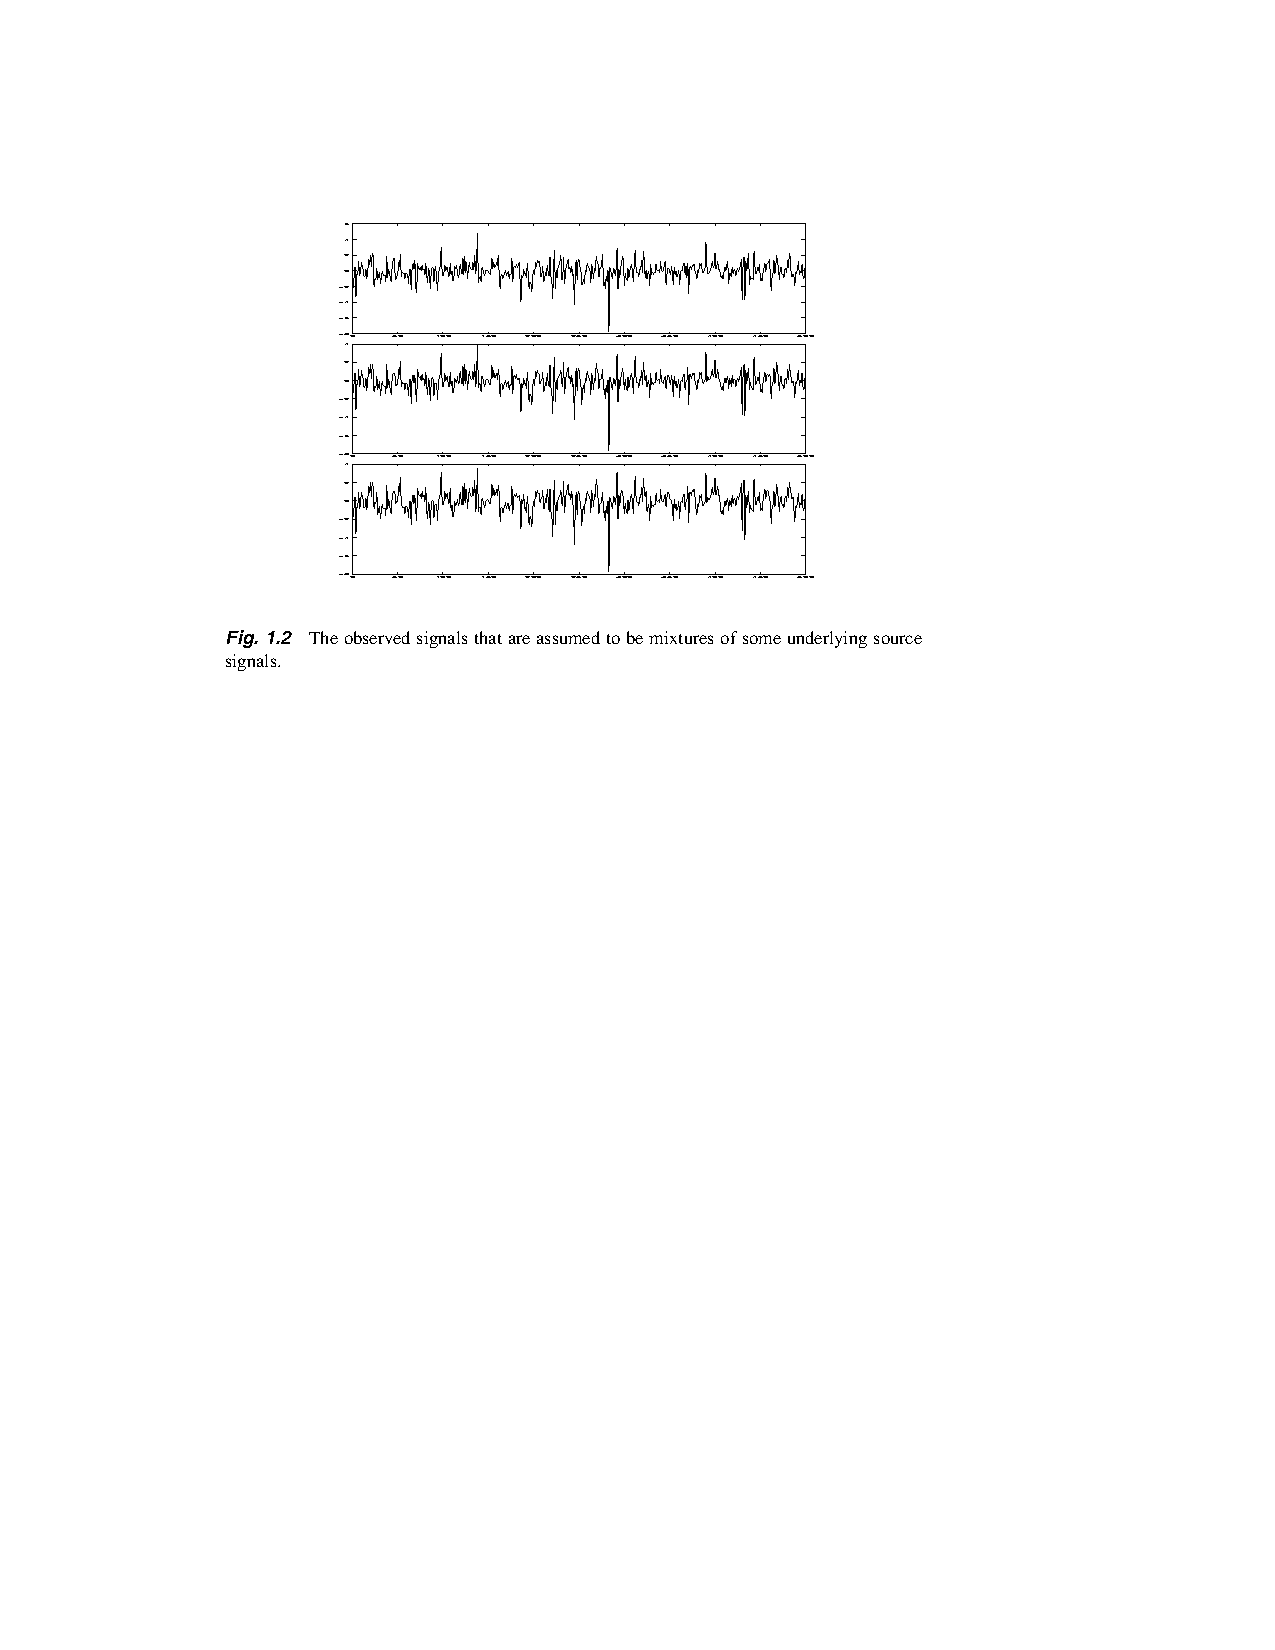
\includegraphics[width=0.3\textwidth]{ICABOOK2001_ObservedSignals}
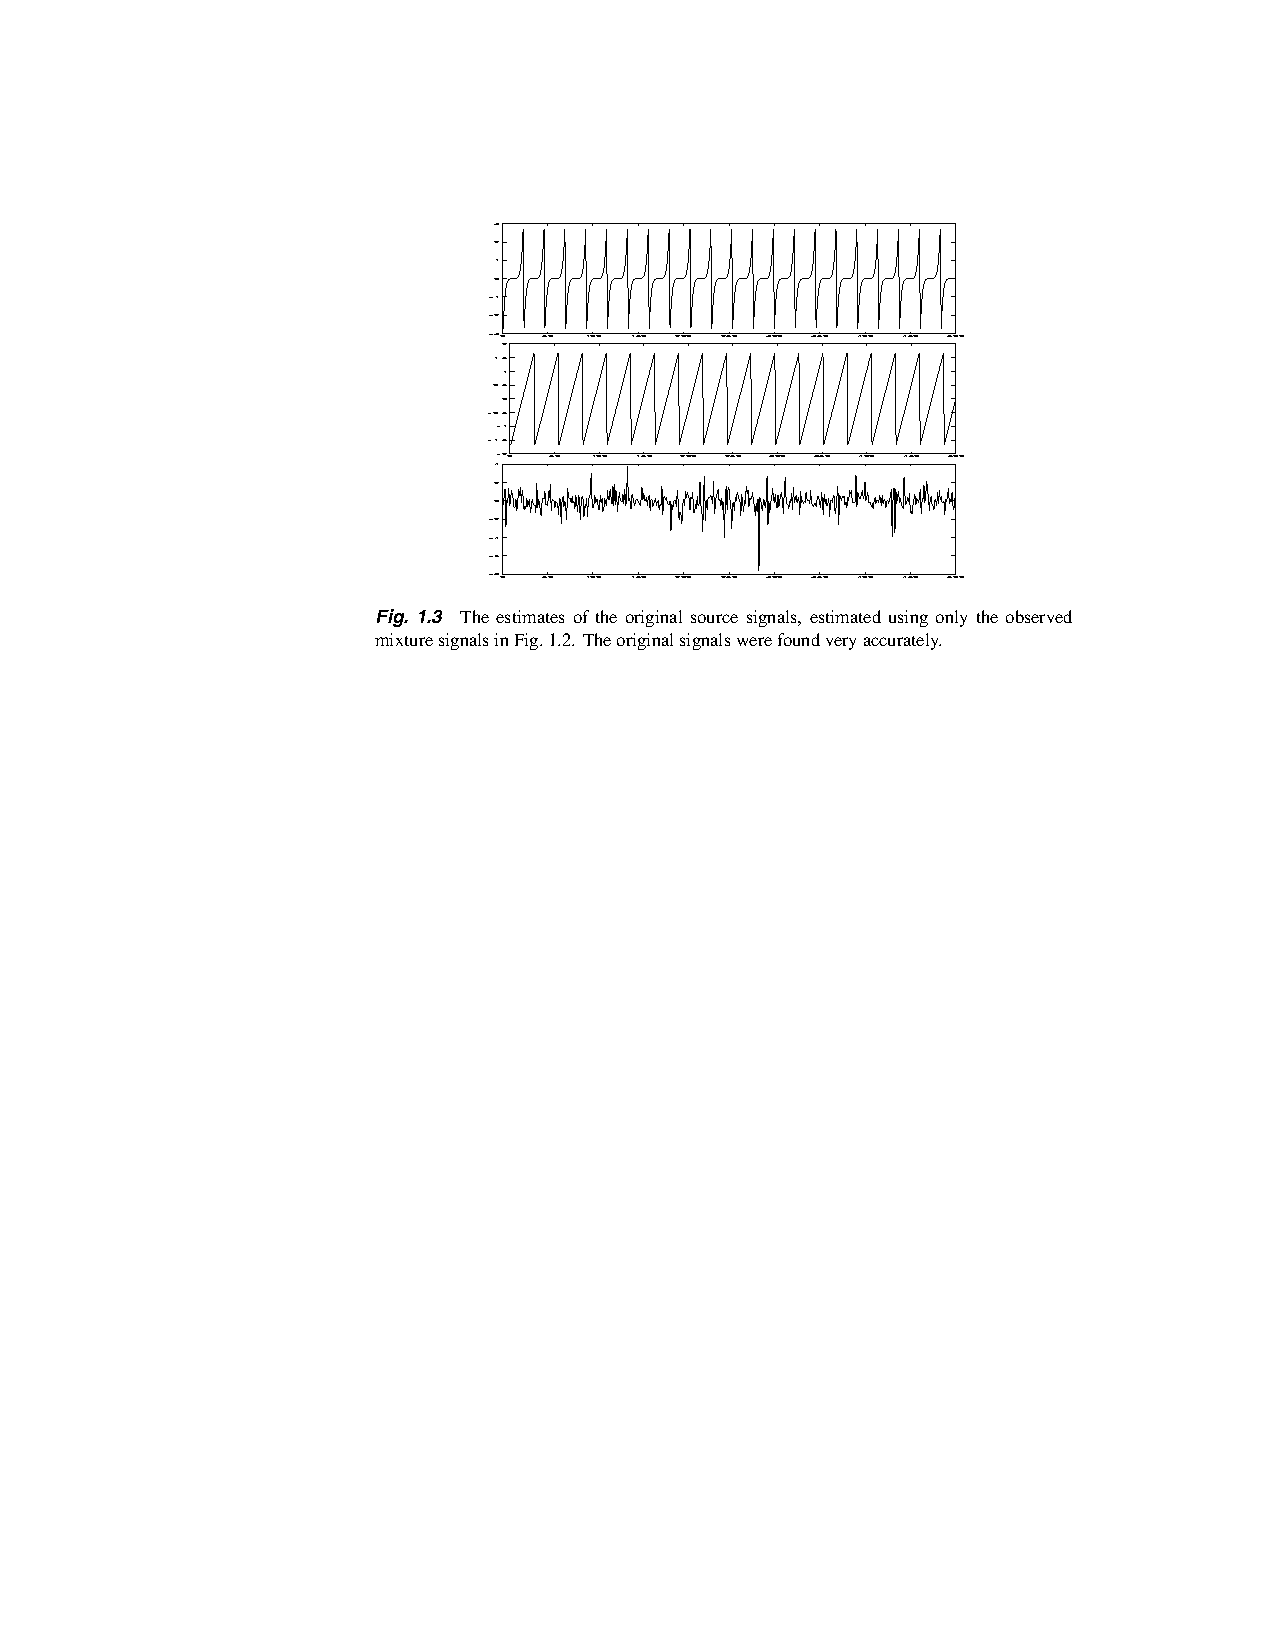
\includegraphics[width=0.3\textwidth]{ICABOOK2001_ReconstructedSignals}
}

\begin{quotation}
\uncover<+->{This leads us to the following definition of ICA [$\dots$]}
\uncover<+->{Given a set of observations of random variables
$(x_1(t),x_2(t),\dots,x_d(t))$, 
where $t$ is the time or sample index, 
assume that they are generated as a linear mixture of \alert{independent components}:}
\uncover<+->{
\[
\begin{pmatrix}
x_1(t)\\x_2(t)\\ \vdots \\ x_d(t)
\end{pmatrix} = A
\begin{pmatrix}
s_1(t)\\s_2(t)\\ \vdots \\ s_d(t)
\end{pmatrix}\,,
\]
where $A$ is some unknown matrix.}
\uncover<+->{%
Independent component analysis now consists of estimating both the matrix $A$ and the $s_i(t)$, when we only observe the $x_i(t)$.}
\end{quotation}
}

\frame{
\bc
\LARGE Good?
\ec
}

\frame{
\frametitle{Independence?}
\bc
\vspace*{-0.45in}
\mbox{}\hspace*{0.5\textwidth}
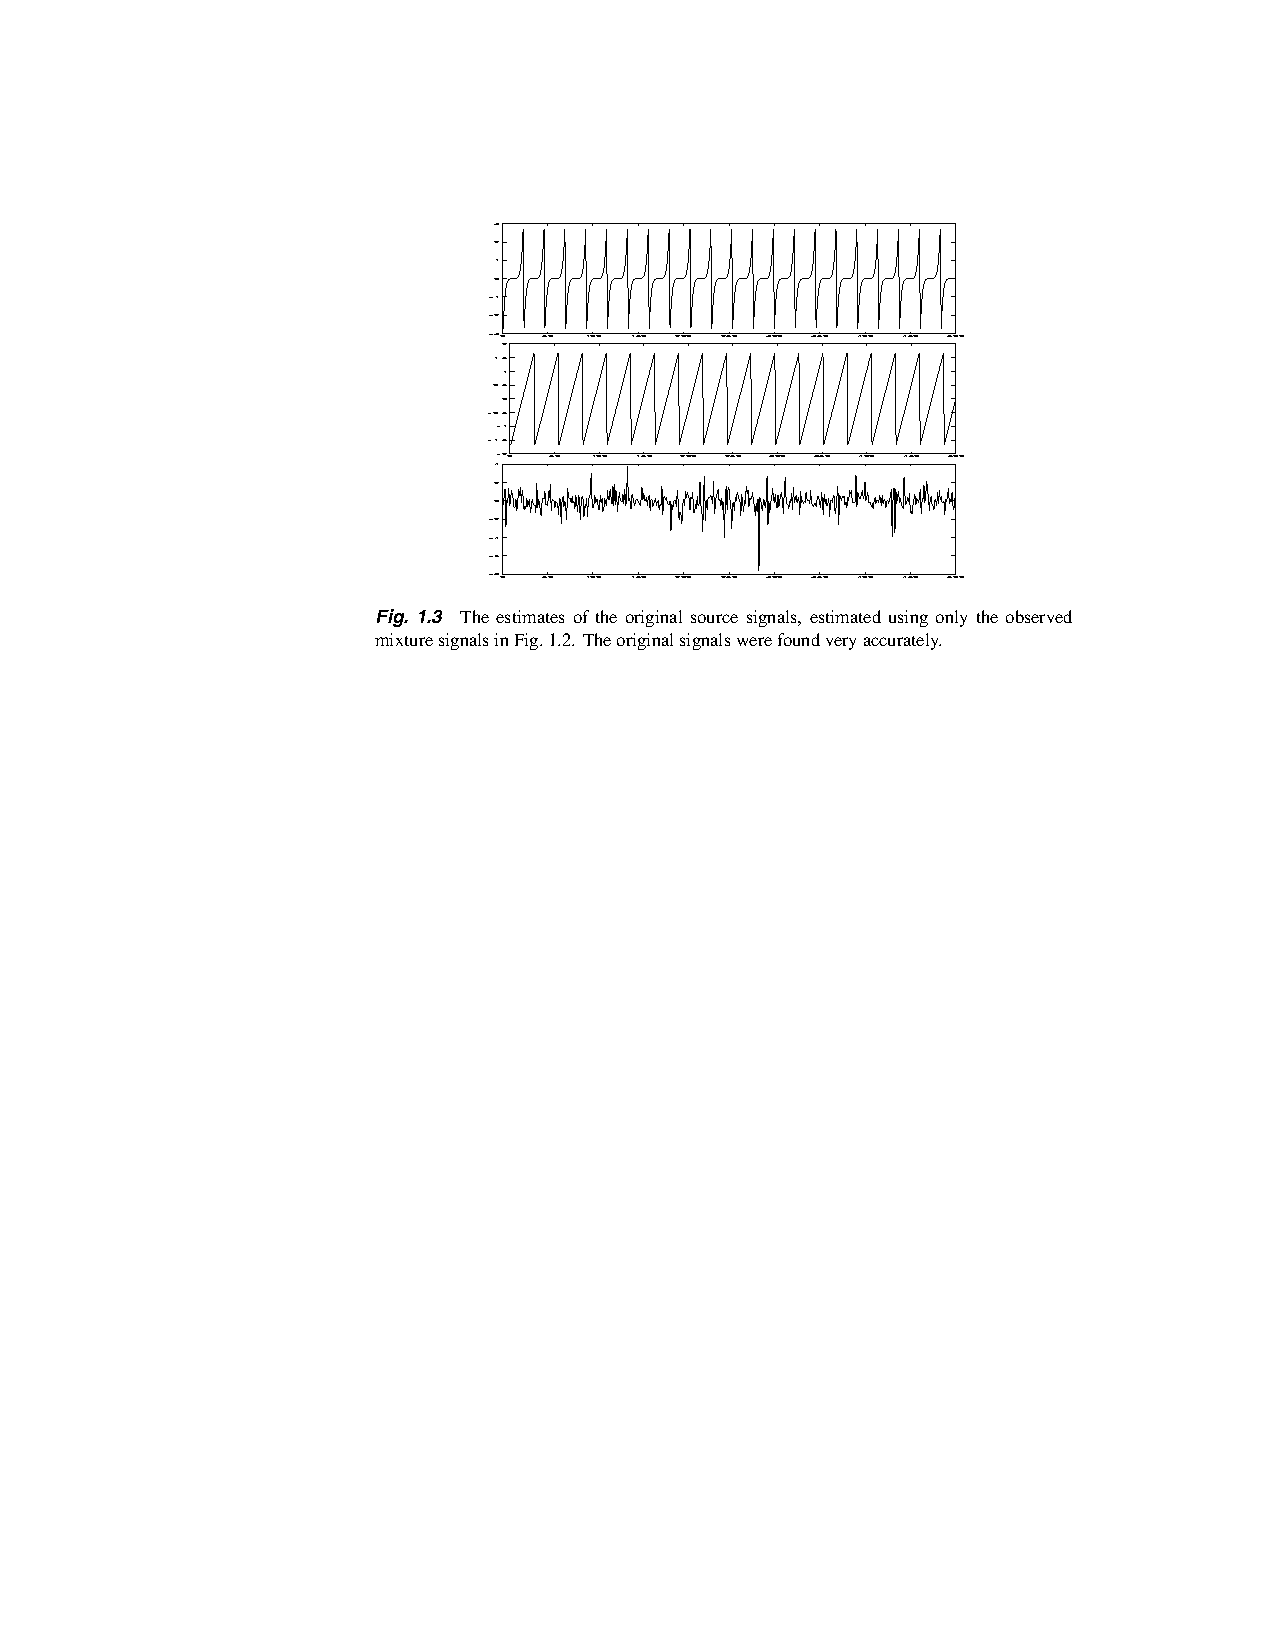
\includegraphics[width=0.45\textwidth]{ICABOOK2001_ReconstructedSignals}
\ec
\bi
\item Is $s_1(t)$ independent of $s_2(t)$? \uncover<+->{Sure!} \uncover<+->{How about $s_1(t)$ and $s_3(t)$?}
\item Any two numbers are independent of each other! 
\uncover<+->{All deterministic signal sources are fine then?}
\item Should we be worried about temporal dependencies? \uncover<+->{No?}
\uncover<+->{What if $s_1(t) = s_1(t+1) = \dots$? }
\item What is ICA then???
\item Leon Bottou: \alert{Can't reduce everything to statistics!}
\item Here: \alert{Let's go beyond statistics!}
\ei
}

\frame{
\frametitle{How to go beyond statistical analysis?}
\begin{enumerate}[<+->]
\item Perform a deterministic analysis of the algorithm, reducing the problem to perturbation analysis
\item Perform statistical analysis on the size of perturbations when necessary or desired
\end{enumerate}

\begin{block}<+->{History}
\bi
\item Online learning (adversarial, regret analysis of learning algorithms) \citet{CBLu06:book}
\item Regression analysis: \citet{vito2006learning}
\item Value function estimation in RL: \citet{PiSze1206}
\item ICA: This work
\ei
\end{block}
}

\subsection{Deterministic ICA}
\begin{frame}{Outline}
\tableofcontents[currentsubsection]
\end{frame}


\frame{
\frametitle{What signals can be separated?}

\bi
\item \uncover<+->{Wrong question!}
\item Better: To what extent can we separate the mixture of some signals?
\ei

\uncover<+->{
Let $[T] = \{1,\dots,T\}$.
Sources:  $s:[T] \to [-C,C]^d$.
}

\uncover<+->{
Let $\nu_T^{(s)}$ be the empirical distribution induced by $s$; for $B\subset [-C,C]^d$,
	\[
	\nu_T^{(s)}(B)=\tfrac{1}{T}|\{t \in [T]: s(\tau) \in B\}|.
	\]
}

\begin{block}<+->{Measure of independence}
%Our independence measure:
	\[
	D_4	= \inf_{\mu} \sup_{f\in\mathcal{F}} \Big|\int f(s)d\nu_T^{(s)} - \int f(s)d\mu(s)\Big|,
	\]
 $\mathcal{F}$: the set of all monomials up to degree $4$;\\
  $\mu$: any product measure.
\end{block}


\uncover<+->{
\textcolor{blue}{Note}:
When $s(t)$ has independent components and $s(1),\dots,s(T)$ are iid,
$D_4 = O(1/\sqrt{T})$.
}
}

\if0
\frame{ \frametitle{Independent Component Analysis (ICA)} 
\bi 
%\item A special case of Blind Source (Signal) Separation;
\onslide<+->
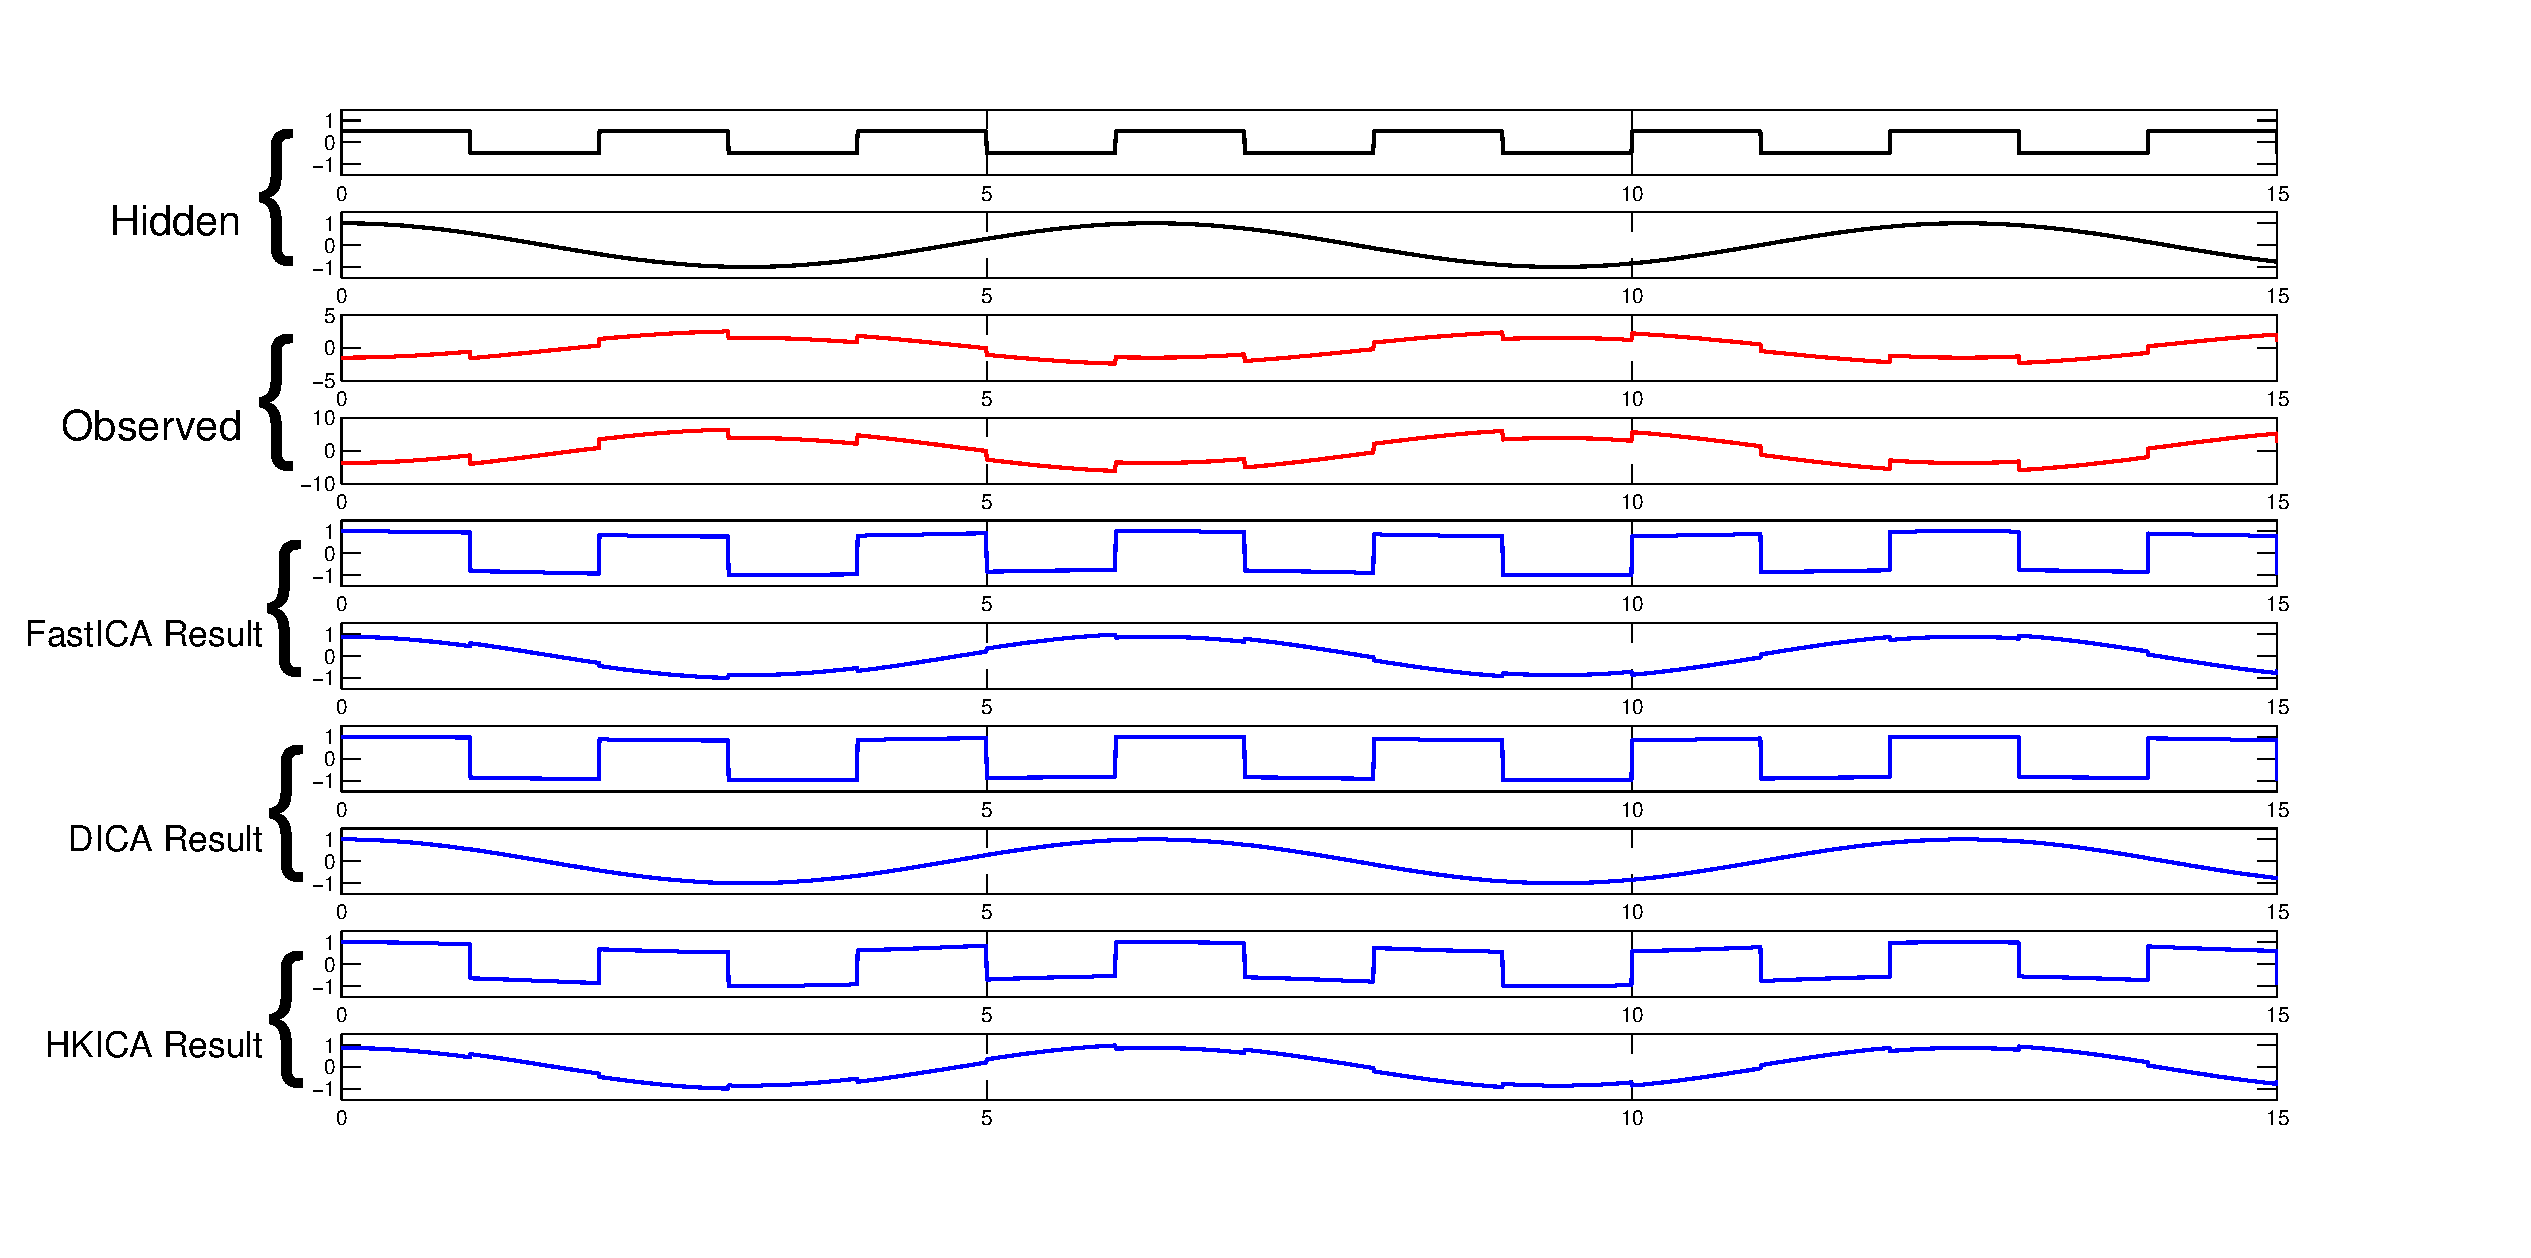
\includegraphics[width=.9\textwidth]{demo}
\ei
}
\fi

\if0
\frame{ \frametitle{Independent Component Analysis (ICA)} 
\bi 
\item  Model: $X = AS + \epsilon$; \\
\onslide<+->
\begin{center}
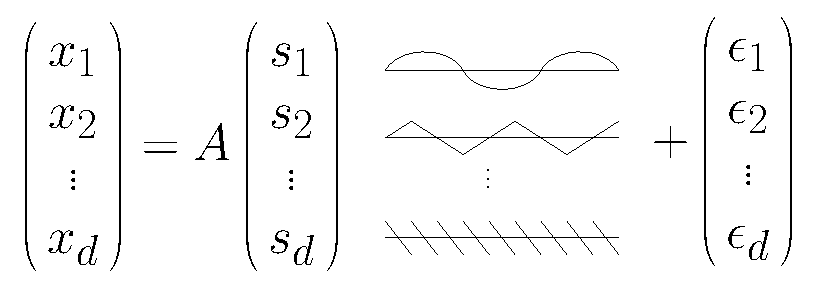
\includegraphics[width=8cm]{ICA_model.eps}
\end{center}
\item $S = (S_1,\ldots, S_d)$ non-Gaussian, $\eps \sim \mathcal{N}(0,\Sigma)$ Gaussian random variables.
\item Goal: Given $T$ independent observations $X(1), \ldots, X(T) \sim X$, reconstruct $A$ up to scaling and permutation. 
\ei
}
\frame{ \frametitle{Independent Component Analysis (ICA)} 
\begin{center}
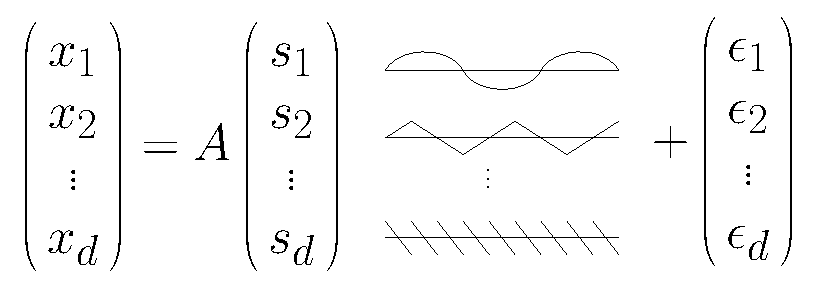
\includegraphics[width=8cm]{ICA_model.eps}
\end{center}
\bi
\item Assumptions:
	\bi
	\item[--] $S_1(t),\ldots, S_d(t)$, $\eps_1(t), \ldots, \eps_d(t)$ are mutually independent for any $t$.
	\vspace{0.3cm}
	\item[--] $A$ is non-singular (for simplicity). 
	\ei
\item Applications: Optical imaging; Telecommunications; Biology; Medicine. 
\ei
}
\fi

\frame{
\frametitle{Goal}
Assuming $x(t) = A s(t) + \eps(t)$, $t=1,\dots, T$;
\\ $\eps(t)$ ``noise''.\\

\medskip

Can we find a method with the following characteristics?

\bi
\setlength{\itemsep}{10pt}
\item[\ds] Universal: No free parameters!
\item[\ds] Efficient:  $\mathrm{poly}(T,d)$ runtime (no dependence on $C$, $A$, $\dots$);
\item[\ds] Robust \& noise-tolerant: $\mathrm{lin}(D_4+1/\sqrt{T})$ accurate in recovering $A$ (with i.i.d. observation noise)?
\ei

\uncover<+->{
Accuracy measure:
\[
d(\hat{A},A) = \inf_{
	 \substack{\pi \in \mathrm{Perm}([d])\\
	 c\in \R^d}} \max_{k} 
	|| c_k A_{:\pi(k)} - A_{:k} ||_2\,.
\]
}
}

\subsection{Has not this been done previously?}
\begin{frame}{Outline}
\tableofcontents[currentsubsection]
\end{frame}

\frame{ 
\frametitle{Previous works with theoretical guarantees} 

\onslide<+->
\citet{SaTsy04,CheBi06} and others: 
\bi
\item No noise
\item Semi-parametrics, ``average derivative estimation'';
\item Asymptotics: $\sqrt{n}$ consistency and efficiency;
\item Why estimate something that is then thrown away? (Also: We'll need conditions on these$\dots$)
\ei
\medskip

\onslide<+->
FastICA by \citet{hyvarinen1999fast}:
\bi
\item Perhaps the most popular ICA algorithm.
\item With probability 1, all local optimizers are desired solutions \citep{wei2014study}, given:
	\begin{itemize}
	\item[--]<2-> infinitely many noiseless samples;
	\item[--]<2-> using kurtosis as the scoring function.
	\end{itemize}
\item[-] Weakness: noisy periodic signals;
\ei

\onslide<+->
%\vspace{1cm}
Moment methods: \citep{frieze1996learning,DHsu2012, arora2012provable,goyal2014fourier}.
}

\frame{ \frametitle{Moment methods}
\bi
\item \citet{frieze1996learning}: 
\bi
\item[-] No noise allowed (also: minor gap fixed by \citet{arora2012provable});
\ei
\item \citet{DHsu2012} (``HKICA''):
\bi
\item[-] No theoretical guarantee stated;
\item[-] If we do the analysis, accuracy will depend on $\gamma_A$; an uncontrolled parameter (see later).
\ei
\item \citet{arora2012provable}:
\bi
\item[-] Free parameter ``$\beta$'', whose choice depends on $||A_{:i}||_2$, while $x\in \{-1,+1\}^d$.
\item[-] Choose either the scale of sources or the scale of the columns of $A$, not both!
\ei
\item Fourier PCA \citep{goyal2014fourier} (FPCA):
\bi
\item[-] Free parameter: Same problem as with \citet{arora2012provable}'s approach.
\ei
%\\
%\quad - If you assume that both the mixing matrix and the sources are bounded with a known bound, 
%the parameter can be chosen.
%\\
\ei

\uncover<+->{\centering \alert{Why care about a free parameters?}}
\uncover<+->{\centering $\dots$ \textcolor{blue}{unsupervised} learning}
%This is unsupervised learning!\\
%Cross-validation is messy at best.
%\end{block}
}


\section{Results}
\begin{frame}{Outline}
\tableofcontents[currentsection]
\end{frame}

\frame{ \frametitle{Result}
There exist a randomized method to estimate $A$ from $(x(t))_{t=1}^T$, with $x(t)=A s(t) + \eps(t)$, $t=1,\dots,T$ s.t.:
\bi
\item The computational complexity is $O(d^3 T)$;
\item With high probability, the output $\hat{A}$ satisfies
	\[
	d(\hat{A},A) \le \theta_1 \min( D_4 + 1/\sqrt{T}, \theta_2 )\,.
	\]
\item Here, $\theta_1,\theta_2$ problem dependent, polynomial in the parameters.
\ei
}


\subsection{Our algorithm: Deterministic ICA}
\begin{frame}{Outline}
\tableofcontents[currentsection]
\end{frame}


\frame{ \frametitle{Hsu-Kakade method (HKICA)} 
\begin{columns}[t]
\column{0.5\textwidth}
\bi
\item[-] For $\eta \in \R^d$, let $f(\eta) = \EEp{(\eta^{\top}x)^4} - 3 \EEp{(\eta^{\top}x)^2}^2$;
\item[-] Choose $\phi$ and $\psi$. \emph{(How?)}
\item[-] Let $T(\phi) = \nabla^2 f(\phi)$. Then 
\[T(\phi) = AK 
\left(
\begin{array}{ccc}
\sigma_1 & & \\ 
    & \ddots & \\
    & & \sigma_d
\end{array} 
\right) 
A^{\top},
\]
where $\sigma_i = \left(\phi^{\top}A_i\right)^2$ and $K$ is some diagonal matrix.
\item[-] Let $M = T(\phi)(T(\psi))^{-1}$.
\ei
\column{0.5\textwidth}
\bi
\item[-] Then 
\[M = A 
\left(
\begin{array}{ccc}
\lambda_1 & & \\ %\left(\frac{\phi^{\top}A_1}{\psi^{\top}A_1}\right)^2 & &\\
    & \ddots & \\
    & & \lambda_d %\left(\frac{\phi^{\top}A_d}{\psi^{\top}A_d}\right)^2\\
\end{array} 
\right) 
A^{-1},
\]
where $\lambda_i = \left(\frac{\phi^{\top}A_i}{\psi^{\top}A_i}\right)^2$.
\item[-] Do an eigen-decomposition of $M$ to recover $A$, assuming all $\lambda_i$'s are distinct.
\item[-] Given finite sample $(x(t))_{t=1}^T$, replace $\mathbb{E}[\cdot]$ with $\mathbb{E}_n[\cdot]$.
\ei

\end{columns}
}

\if0
\frame{ \frametitle{Hsu-Kakade method (HKICA)} 
\bi
\item[-] Let $M = T(\phi)(T(\psi))^{-1}$. Then 
\[M = A 
\left(
\begin{array}{ccc}
\lambda_1 & & \\ %\left(\frac{\phi^{\top}A_1}{\psi^{\top}A_1}\right)^2 & &\\
    & \ddots & \\
    & & \lambda_d %\left(\frac{\phi^{\top}A_d}{\psi^{\top}A_d}\right)^2\\
\end{array} 
\right) 
A^{-1},
\]
where $\lambda_i = \left(\frac{\phi^{\top}A_i}{\psi^{\top}A_i}\right)^2$.
\item[-] Do an eigen-decomposition of $M$ to recover $A$, assuming all $\lambda_i$'s are distinct.
\item[-] Given $(x(t))_{t=1}^T$, replace $\EE{\cdot}$ with $\mathbb{E}_n{\cdot}$.
\ei
}
\fi

\frame{ \frametitle{Our issue with the HK method}
{\large{Problem: Minimal gap of the eigenvalues.}}			
\bi
\item Theoretical analysis shows that the performance depends on $\gamma_A^{-1}$, where
	\[
	\gamma_A = \min_{i\neq j} \left\vert \lambda_i - \lambda_j\right \vert.
	\]
\item $\gamma_A$ is not yet well understood%
\footnote{Is $\gamma_A^{-1}$ polynomially bounded in $d$?}
%\item[] in particular, it is not known whether $\gamma_A^{-1} = \mathrm{Poly}(d,A)$\,.
\ei
\bigskip

\uncover<+->{
\centering 
\Large 
\alert{Goal}: Avoid dependency on $\gamma_A^{-1}$!
}
}

\frame{ \frametitle{Our method: Deterministic ICA (DICA)}
\bi
\item[--] Inspired by \citet{arora2012provable} and \citet{frieze1996learning};
\item[--] Sample $\psi$, $\phi_1$ and $\phi_2$ independently from standard normal distribution.
\item[--] Calculate $\nabla^2 f(\psi)$ and $B$ such that $\nabla^2 f(\psi) = BB^{\top}$.%
{\footnote{
\uncover<+->{Recall: $f(\eta) = \EEp{(\eta^{\top}x)^4} - 3 \EEp{(\eta^{\top}x)^2}^2$}}}
\item[--] Calculate $T(\phi_1) = \nabla^2 f(B^{-\top}\phi_1)$ and $T(\phi_2) = \nabla^2 f(B^{-\top}\phi_2)$.
\item[--] Calculate $M = T(\phi_1)(T(\phi_2))^{-1}$.
	\[
	M = R \,\mathrm{diag}\left( \tilde{\lambda}_1, \ldots, \tilde{\lambda}_d \right)R^{\top},
	\]
	where $\tilde{\lambda}_i = \left(\frac{\phi_1^{\top}R_i}{\phi_2^{\top}R_i}\right)^2$ and $R$ is some \alert{orthonormal} matrix
	s.t. \alert{$A = BR$}.
\item[--] Do an eigen-decomposition of $M$ to recover $R$.
\item[--] Return $\hat{A} = BR$ as an estimate of $A$. 
\ei
}

\frame{ \frametitle{Our method: Deterministic ICA (DICA)}
\bi
\item The reconstruction error is proportional to $\gamma_R^{-1}$, where 
	\[ 
	\gamma_R = \min_{i\neq j} \left\vert \tilde{\lambda}_i - \tilde{\lambda}_j\right \vert = \min_{i\neq j} \left\vert \left(\frac{\phi_1^{\top}R_i}{\phi_2^{\top}R_i}\right)^2
	 - \left(\frac{\phi_1^{\top}R_j}{\phi_2^{\top}R_j}\right)^2\right\vert.
	\]
	\bi
	\item[--] $\{\phi_1^{\top}R_1,\ldots, \phi_1^{\top}R_d, \phi_2^{\top}R_1,\ldots, \phi_2^{\top}R_d \}$ are independent standard normal variables.
	\item[--] No dependency on $A$.
	\item[--] Can be reduced to the minimal spacing of Cauchy random variables.
	\ei
\item Recursive version is also developed in the paper, based on the idea of \citet{vempala2014max}.
\ei
}

\section{Empirical Illustration}
\begin{frame}{Outline}
\tableofcontents[currentsection]
\end{frame}

\frame{ \frametitle{Setting}
\begin{columns}[t]
\column{0.5\textwidth}
\uncover<+->{Questions:}
\bi
	\item Does noise matter?
		\bi
		\item[-] Additive Gaussian noise with std $=0.3$.
		\ei
	\item Does coherence matter? 
		\bi 
		\item[-] $A_1$: Gaussian matrix; $A_4$: more coherent matrix.
		\ei
	\item Do the recursive versions improve the results?
\ei
\column{0.5\textwidth}
\uncover<+->{Algorithms:}
\bi
	\item FastICA  \citep{szabo12separation};
	\item HKICA/HKICA.R; 
	\item (recursive) FPCA due to \citet{vempala2014max};
%	\item<1-> Random guessing (Random).
	\\ \mbox{}\\
	\item DICA/DICA.R; 
	\item MDICA/MDICA.R (heuristic version of DICA)
\ei
\end{columns}

}

\frame{
\frametitle{Sources}

Noise-free BPSK sources, $T=20,000$:
\bc
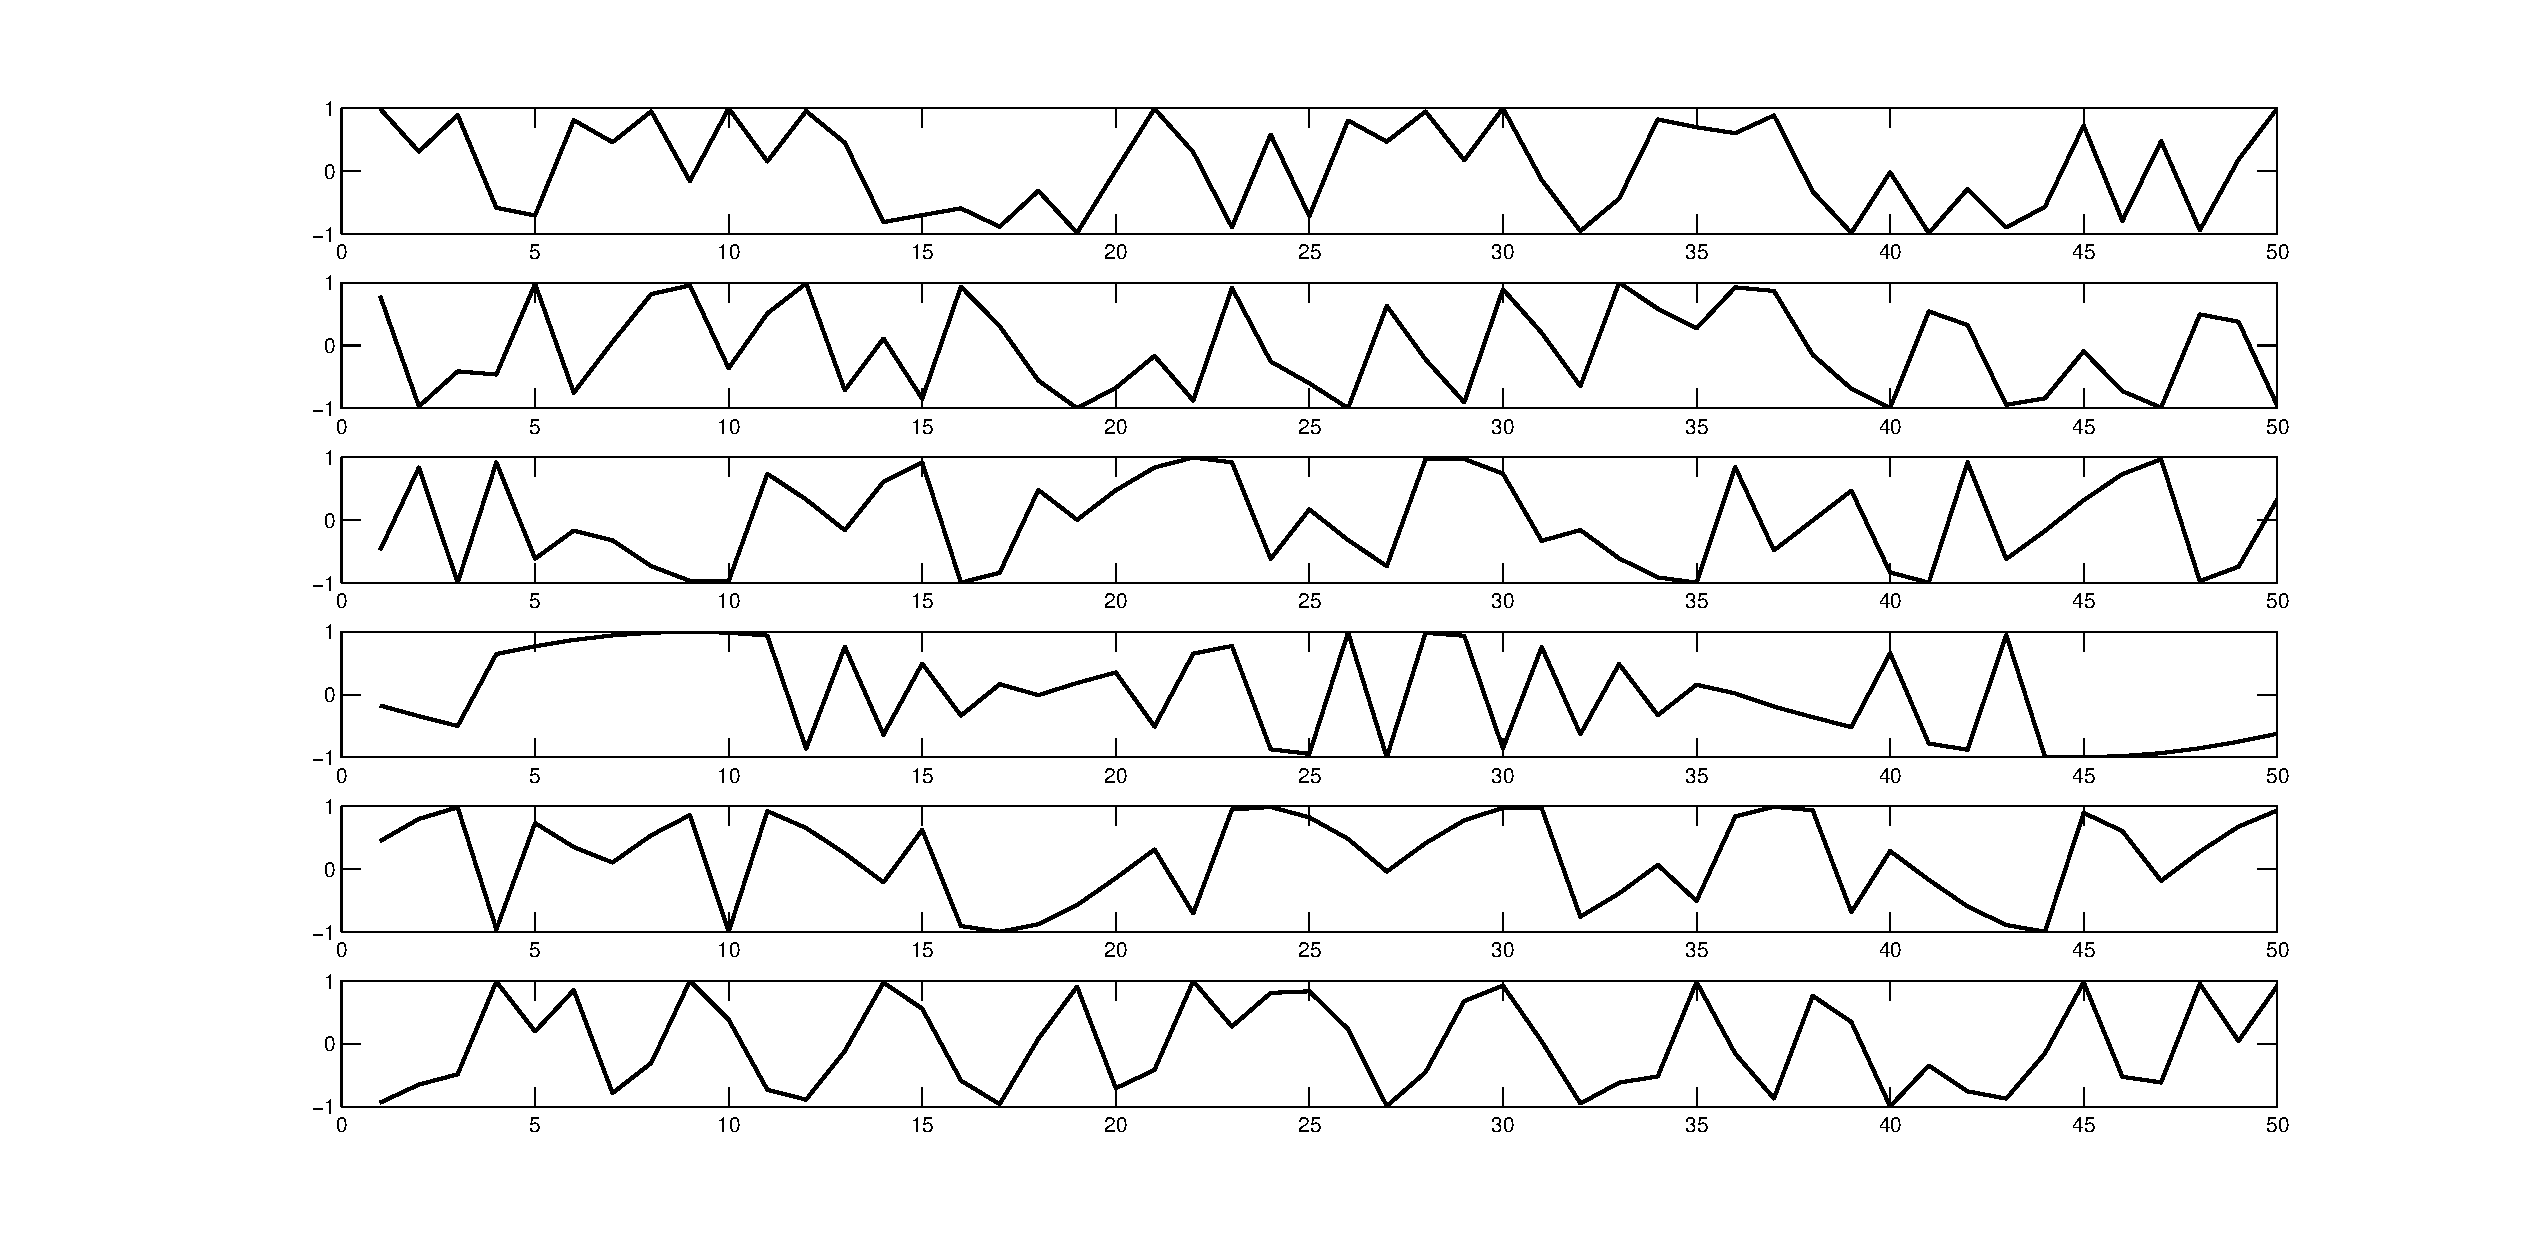
\includegraphics[width=0.5\textwidth]{Diagrams/Hidden-noisefree}
\ec

Noisy BPSK sources:
\bc
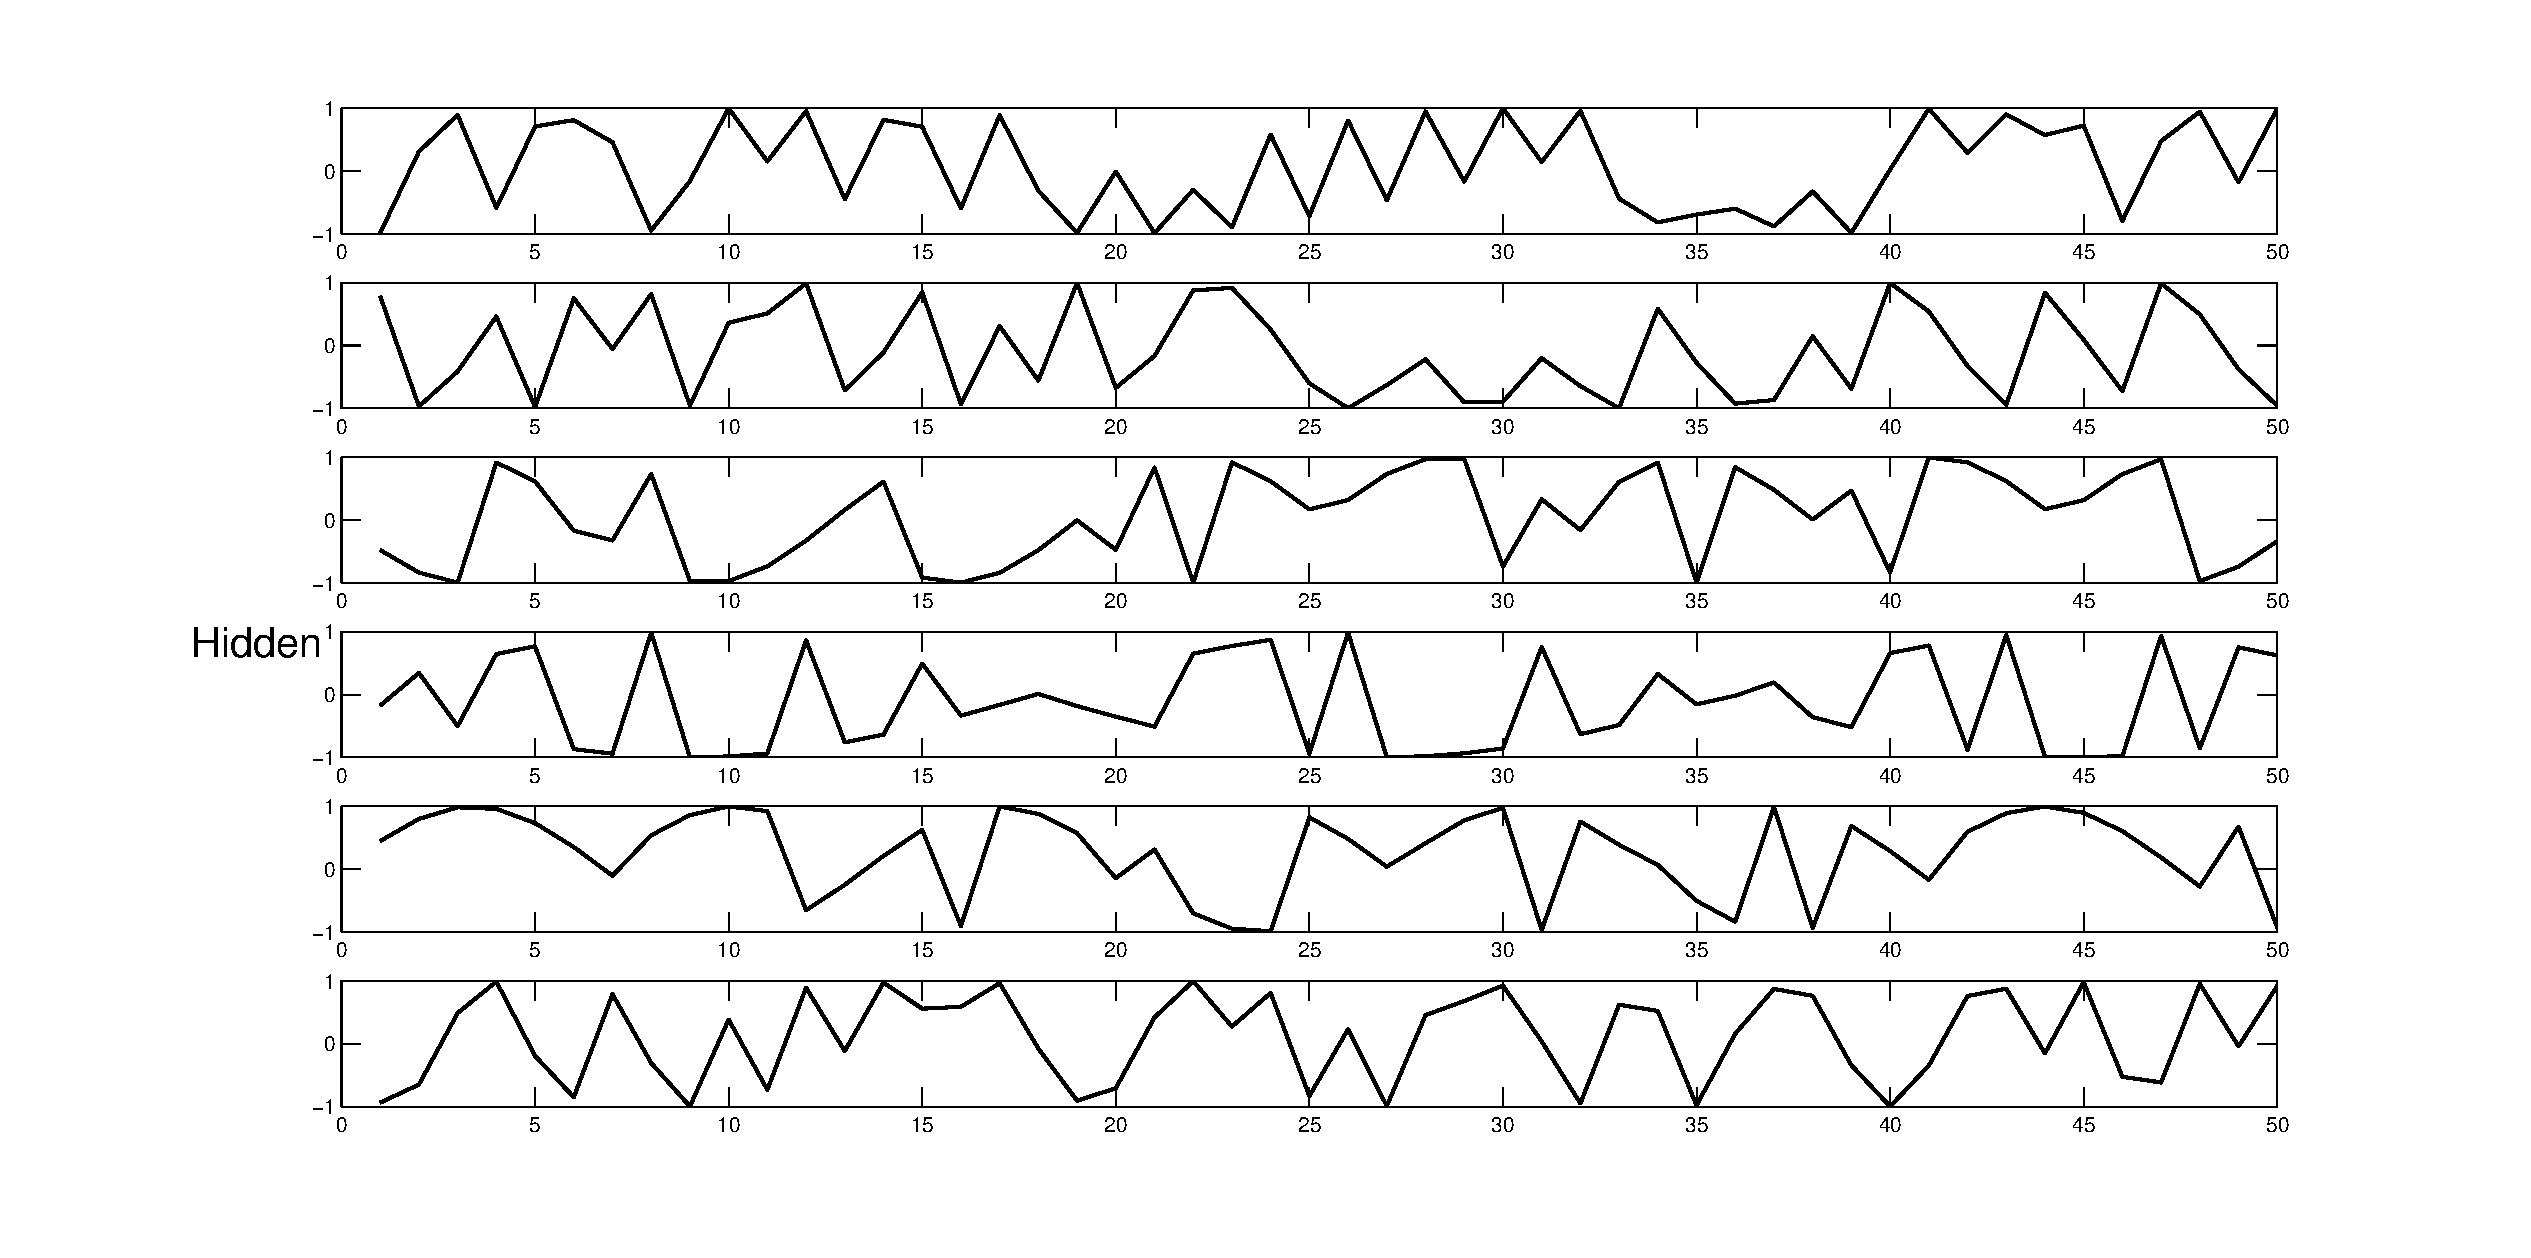
\includegraphics[width=0.5\textwidth]{Diagrams/Hidden-noisy}
\ec
}

\frame{
\frametitle{Observations}

Noise-free observation:
\bc
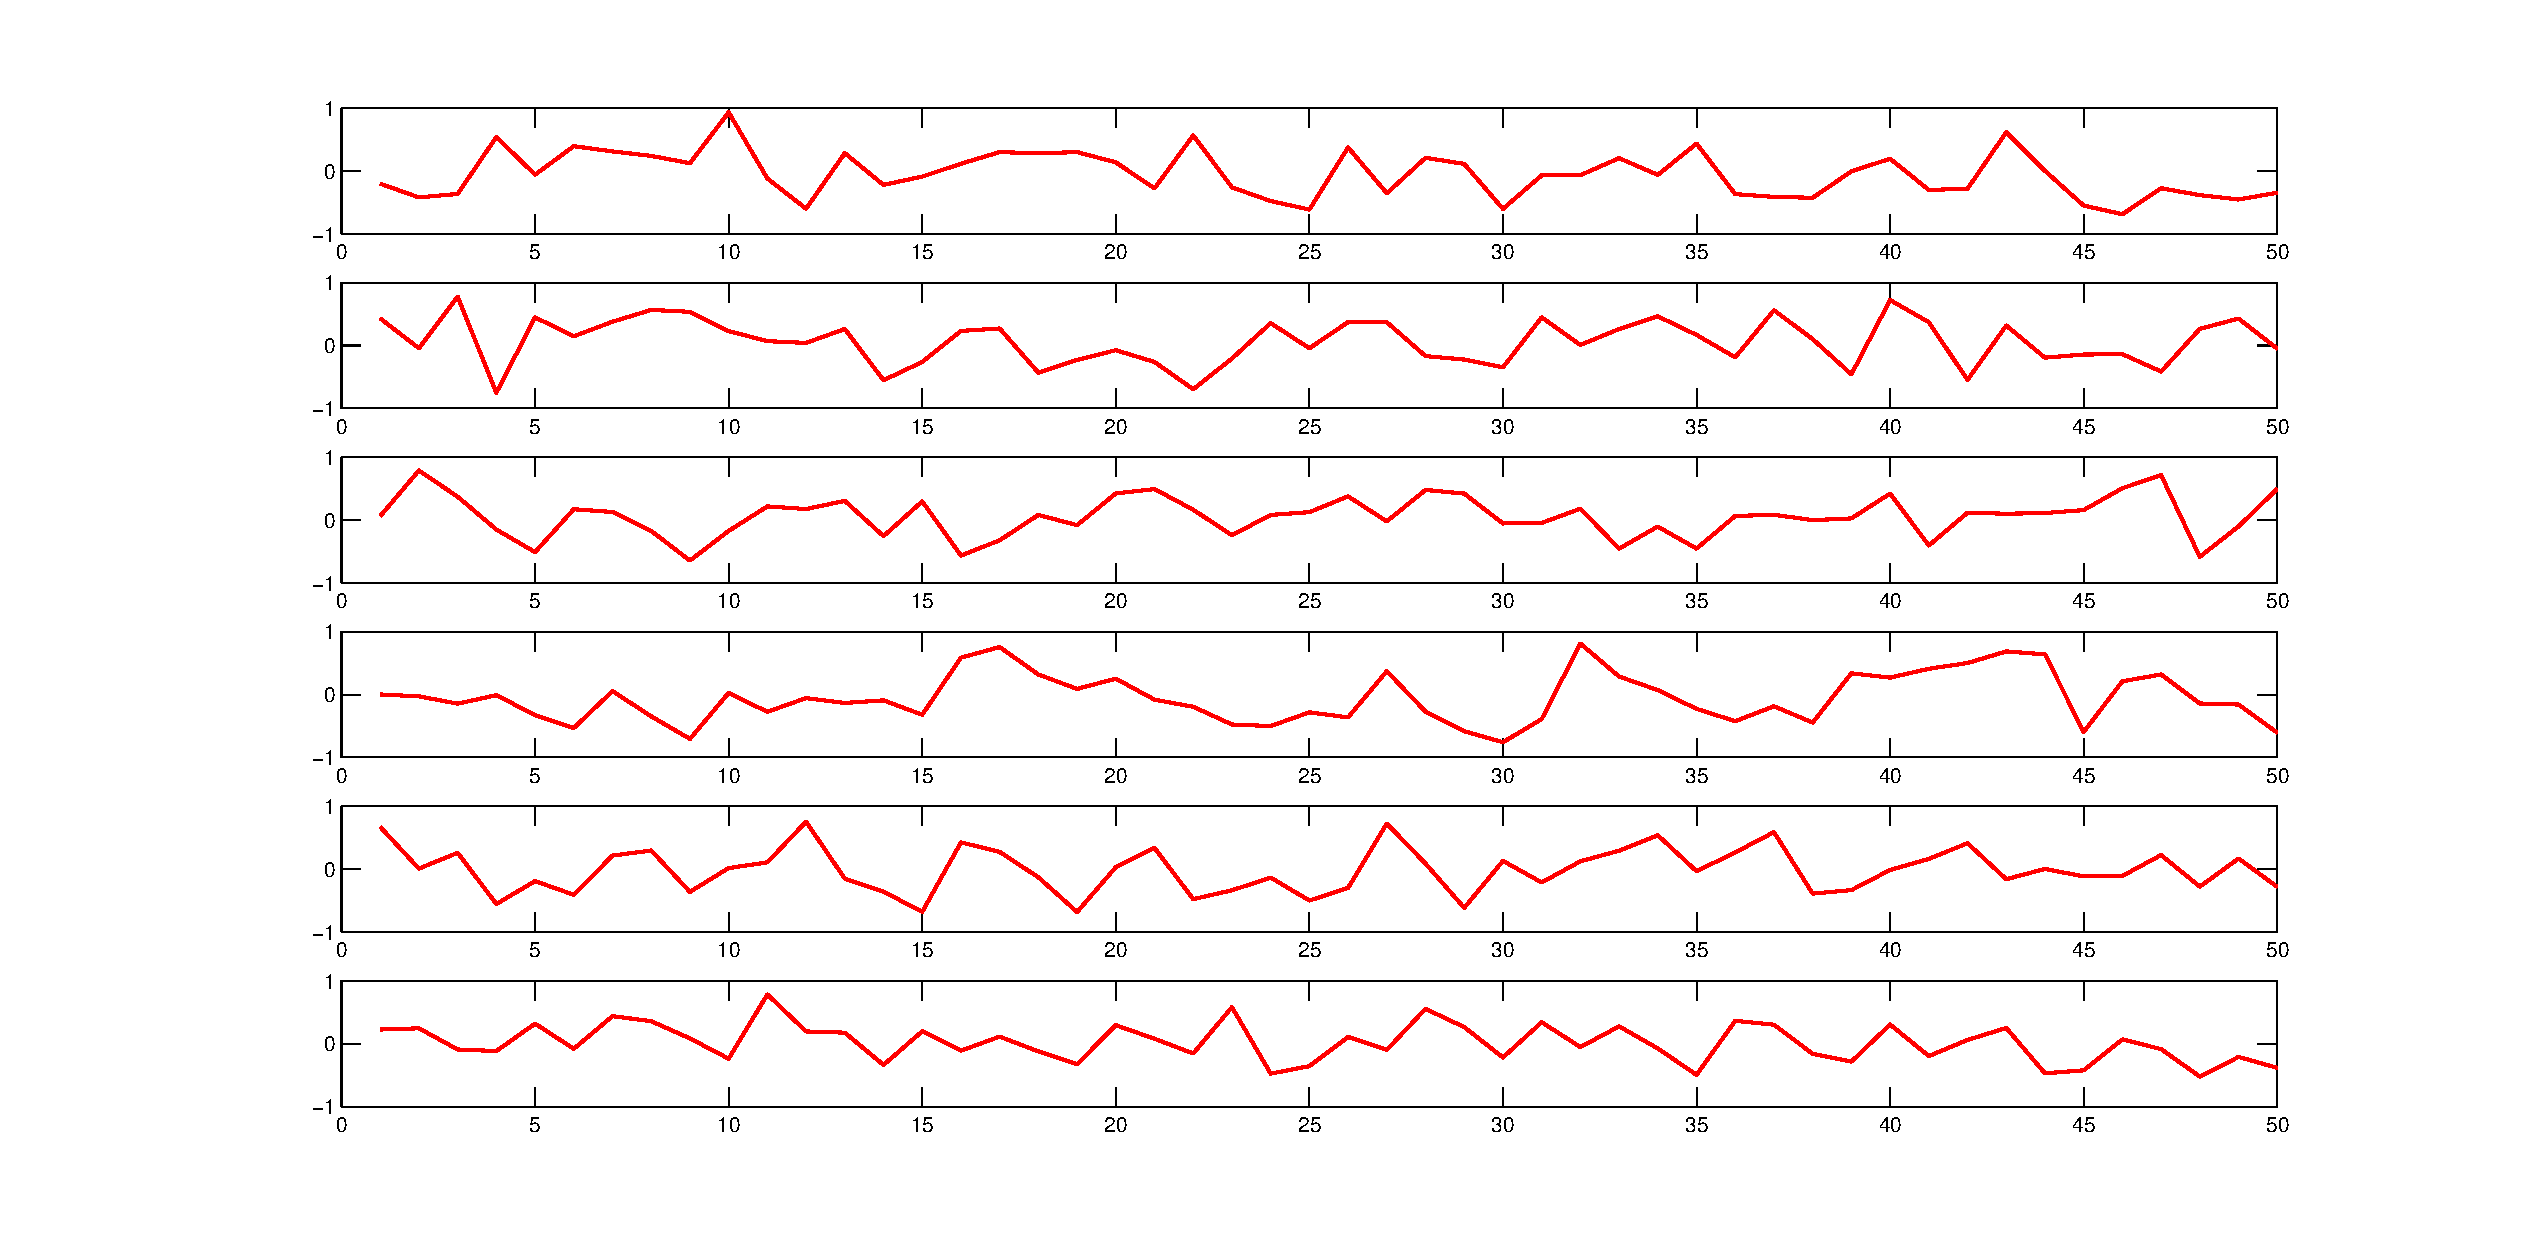
\includegraphics[width=0.5\textwidth]{Diagrams/Observed-noisefree}
\ec

Noisy observation:
\bc
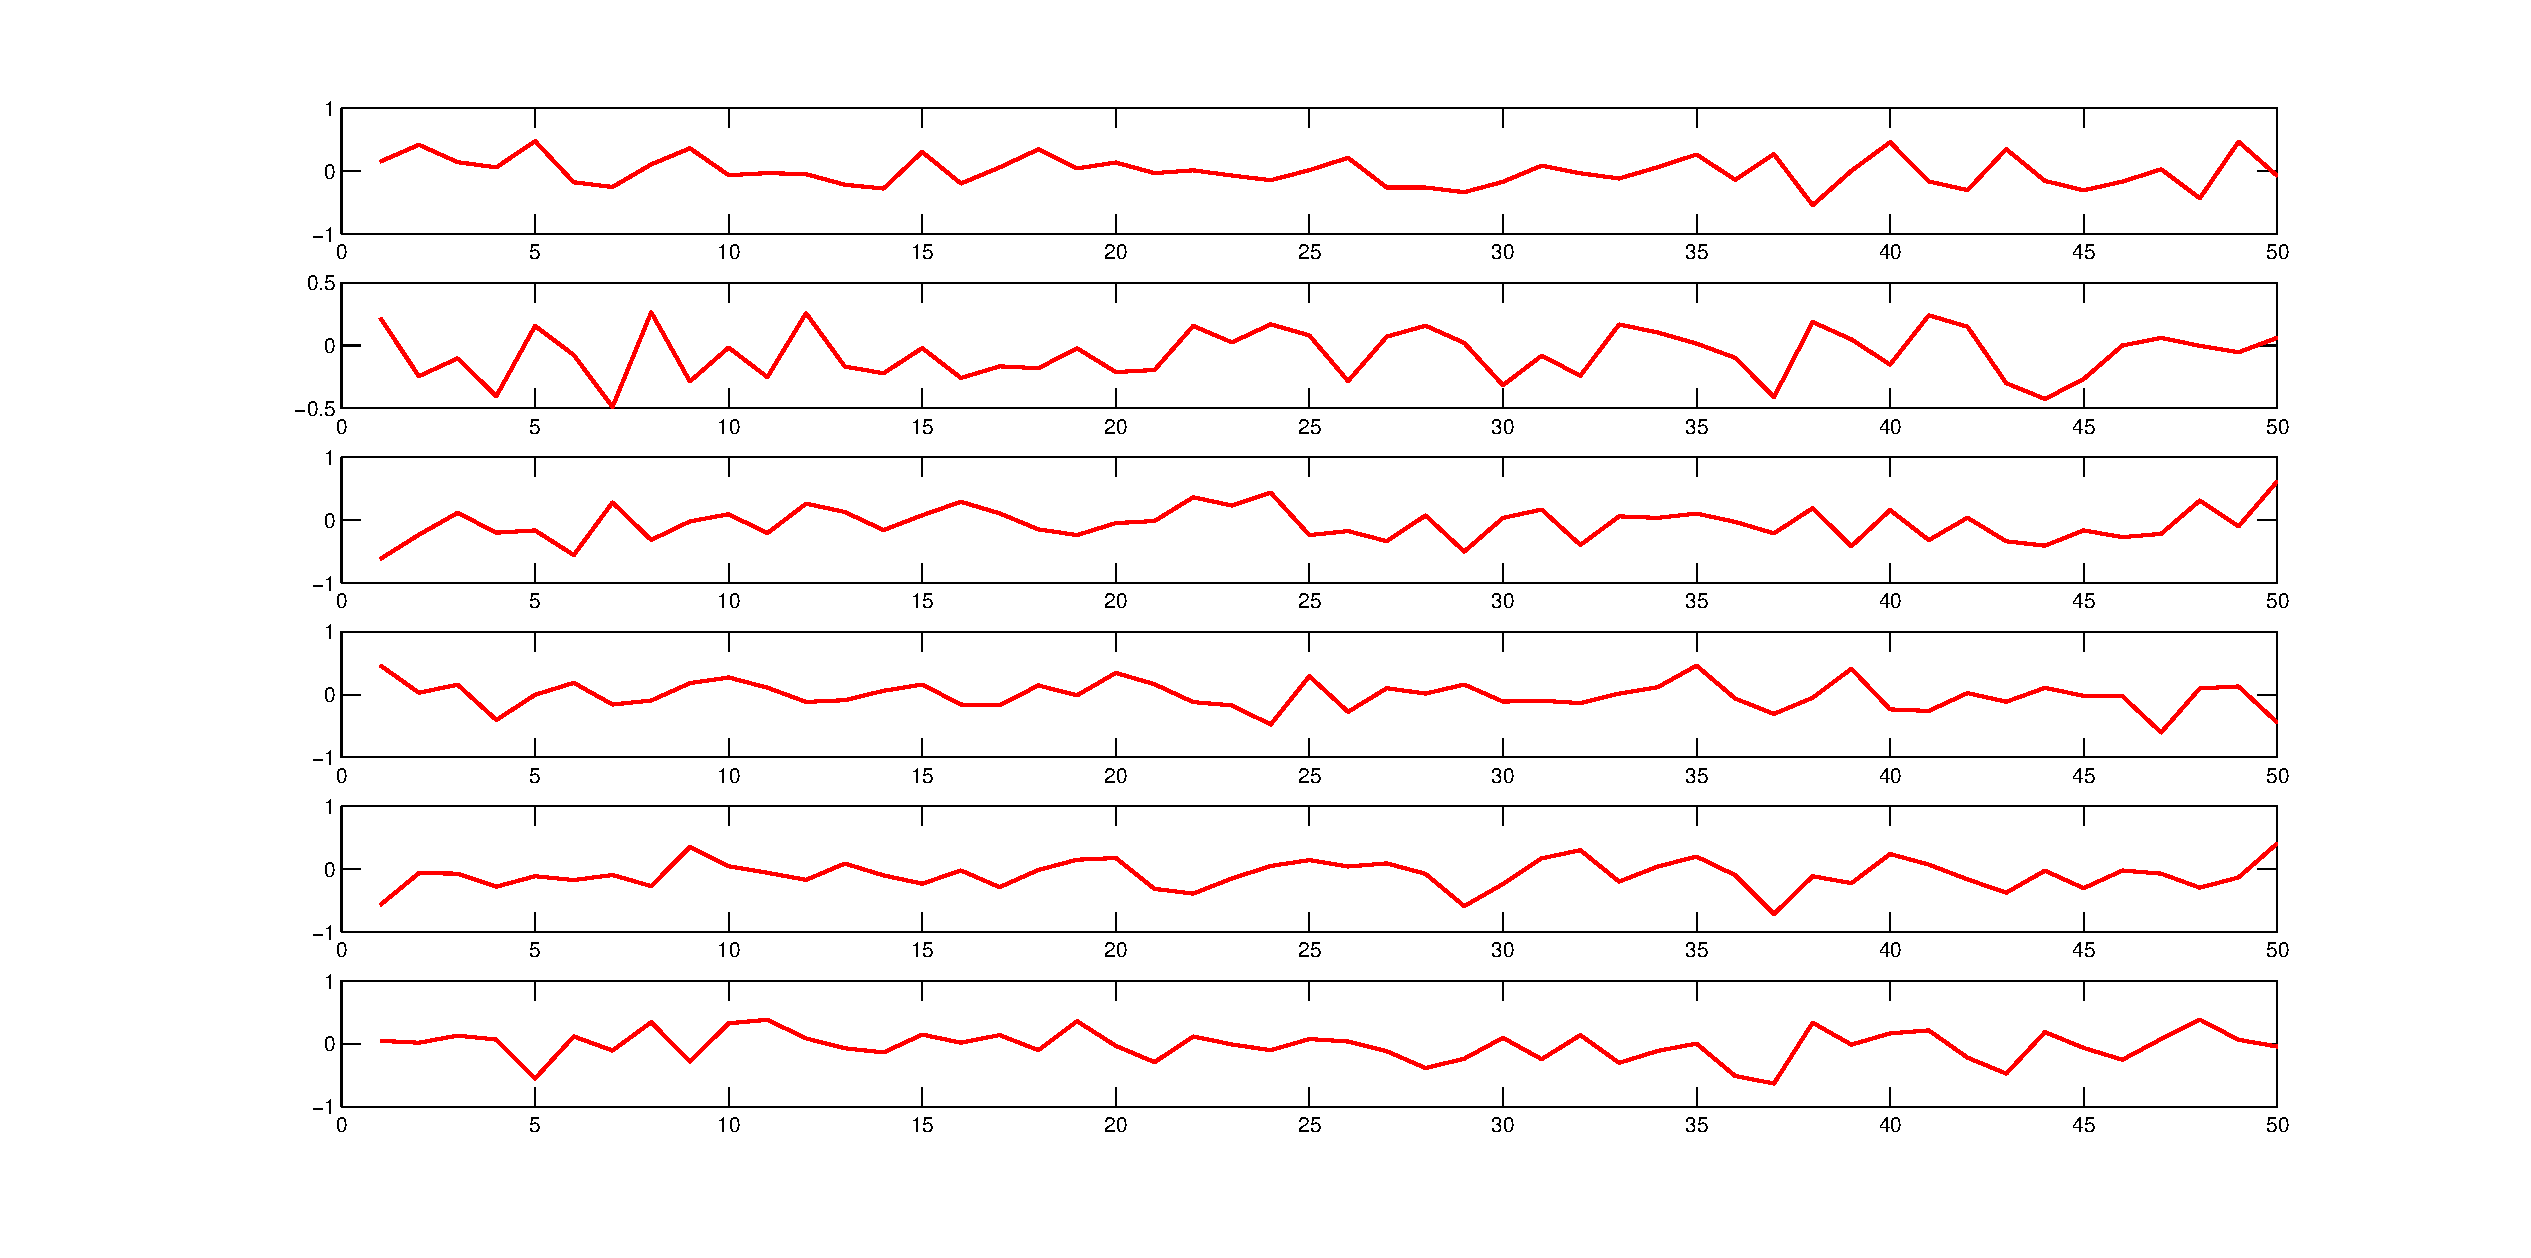
\includegraphics[width=0.5\textwidth]{Diagrams/Observed-noisy}
\ec

}

\frame{
\frametitle{Example reconstructions: Noise-free case}
Noise-free BPSK sources:
\bc
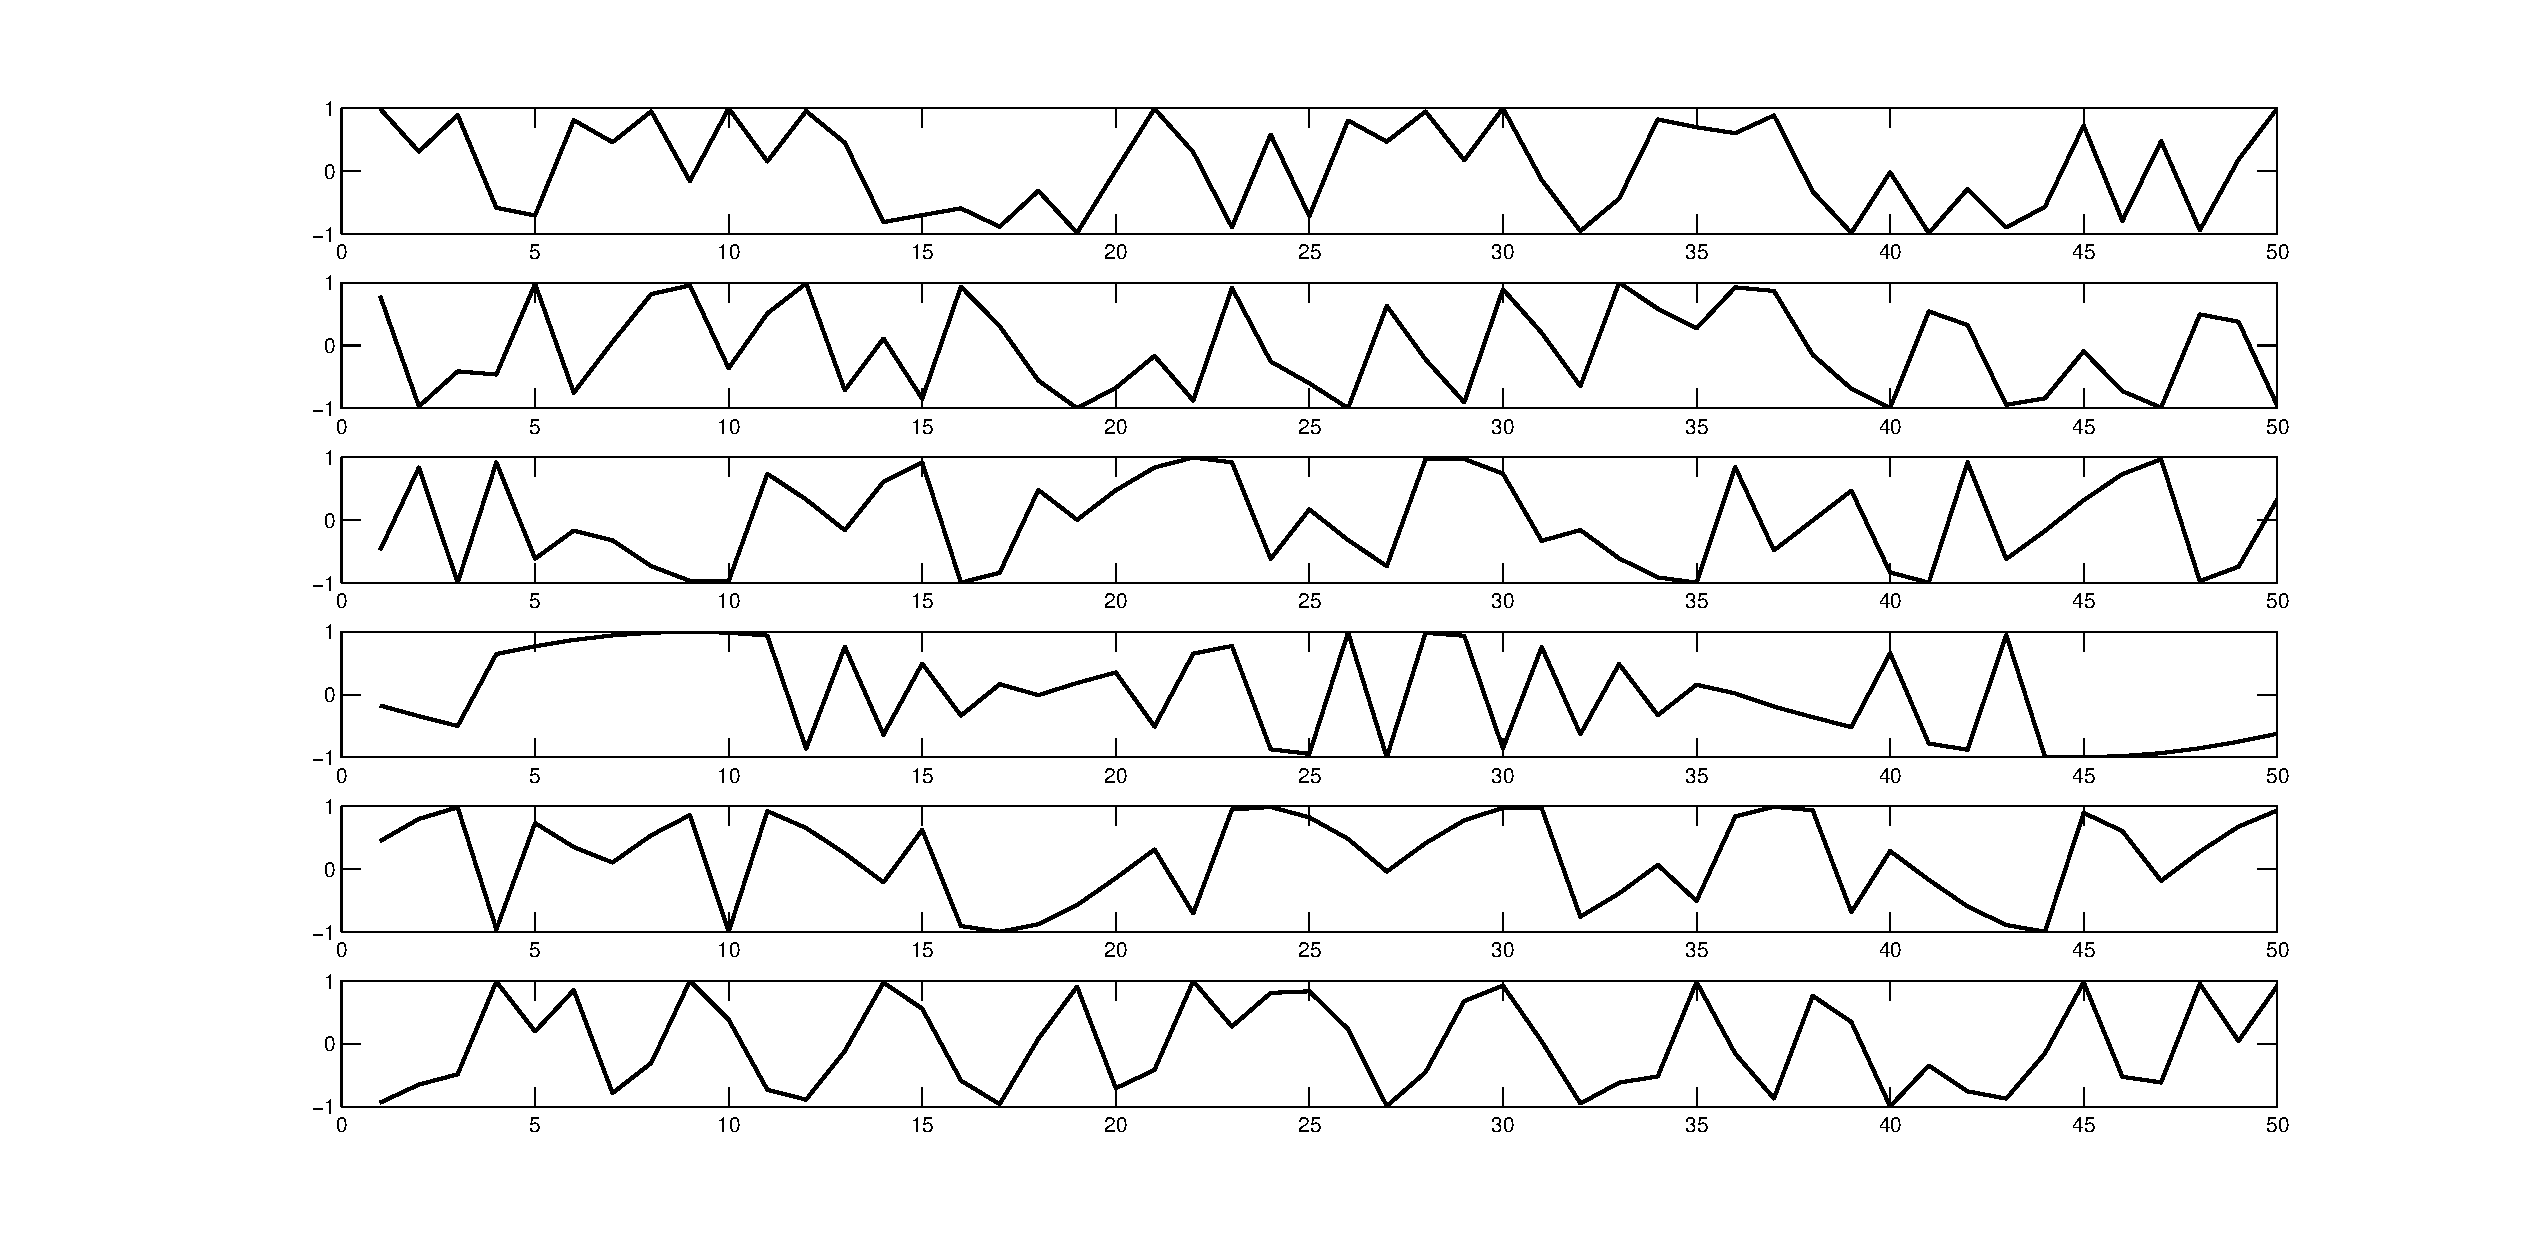
\includegraphics[width=0.5\textwidth]{Diagrams/Hidden-noisefree}
\ec

Reconstruction:
\bc
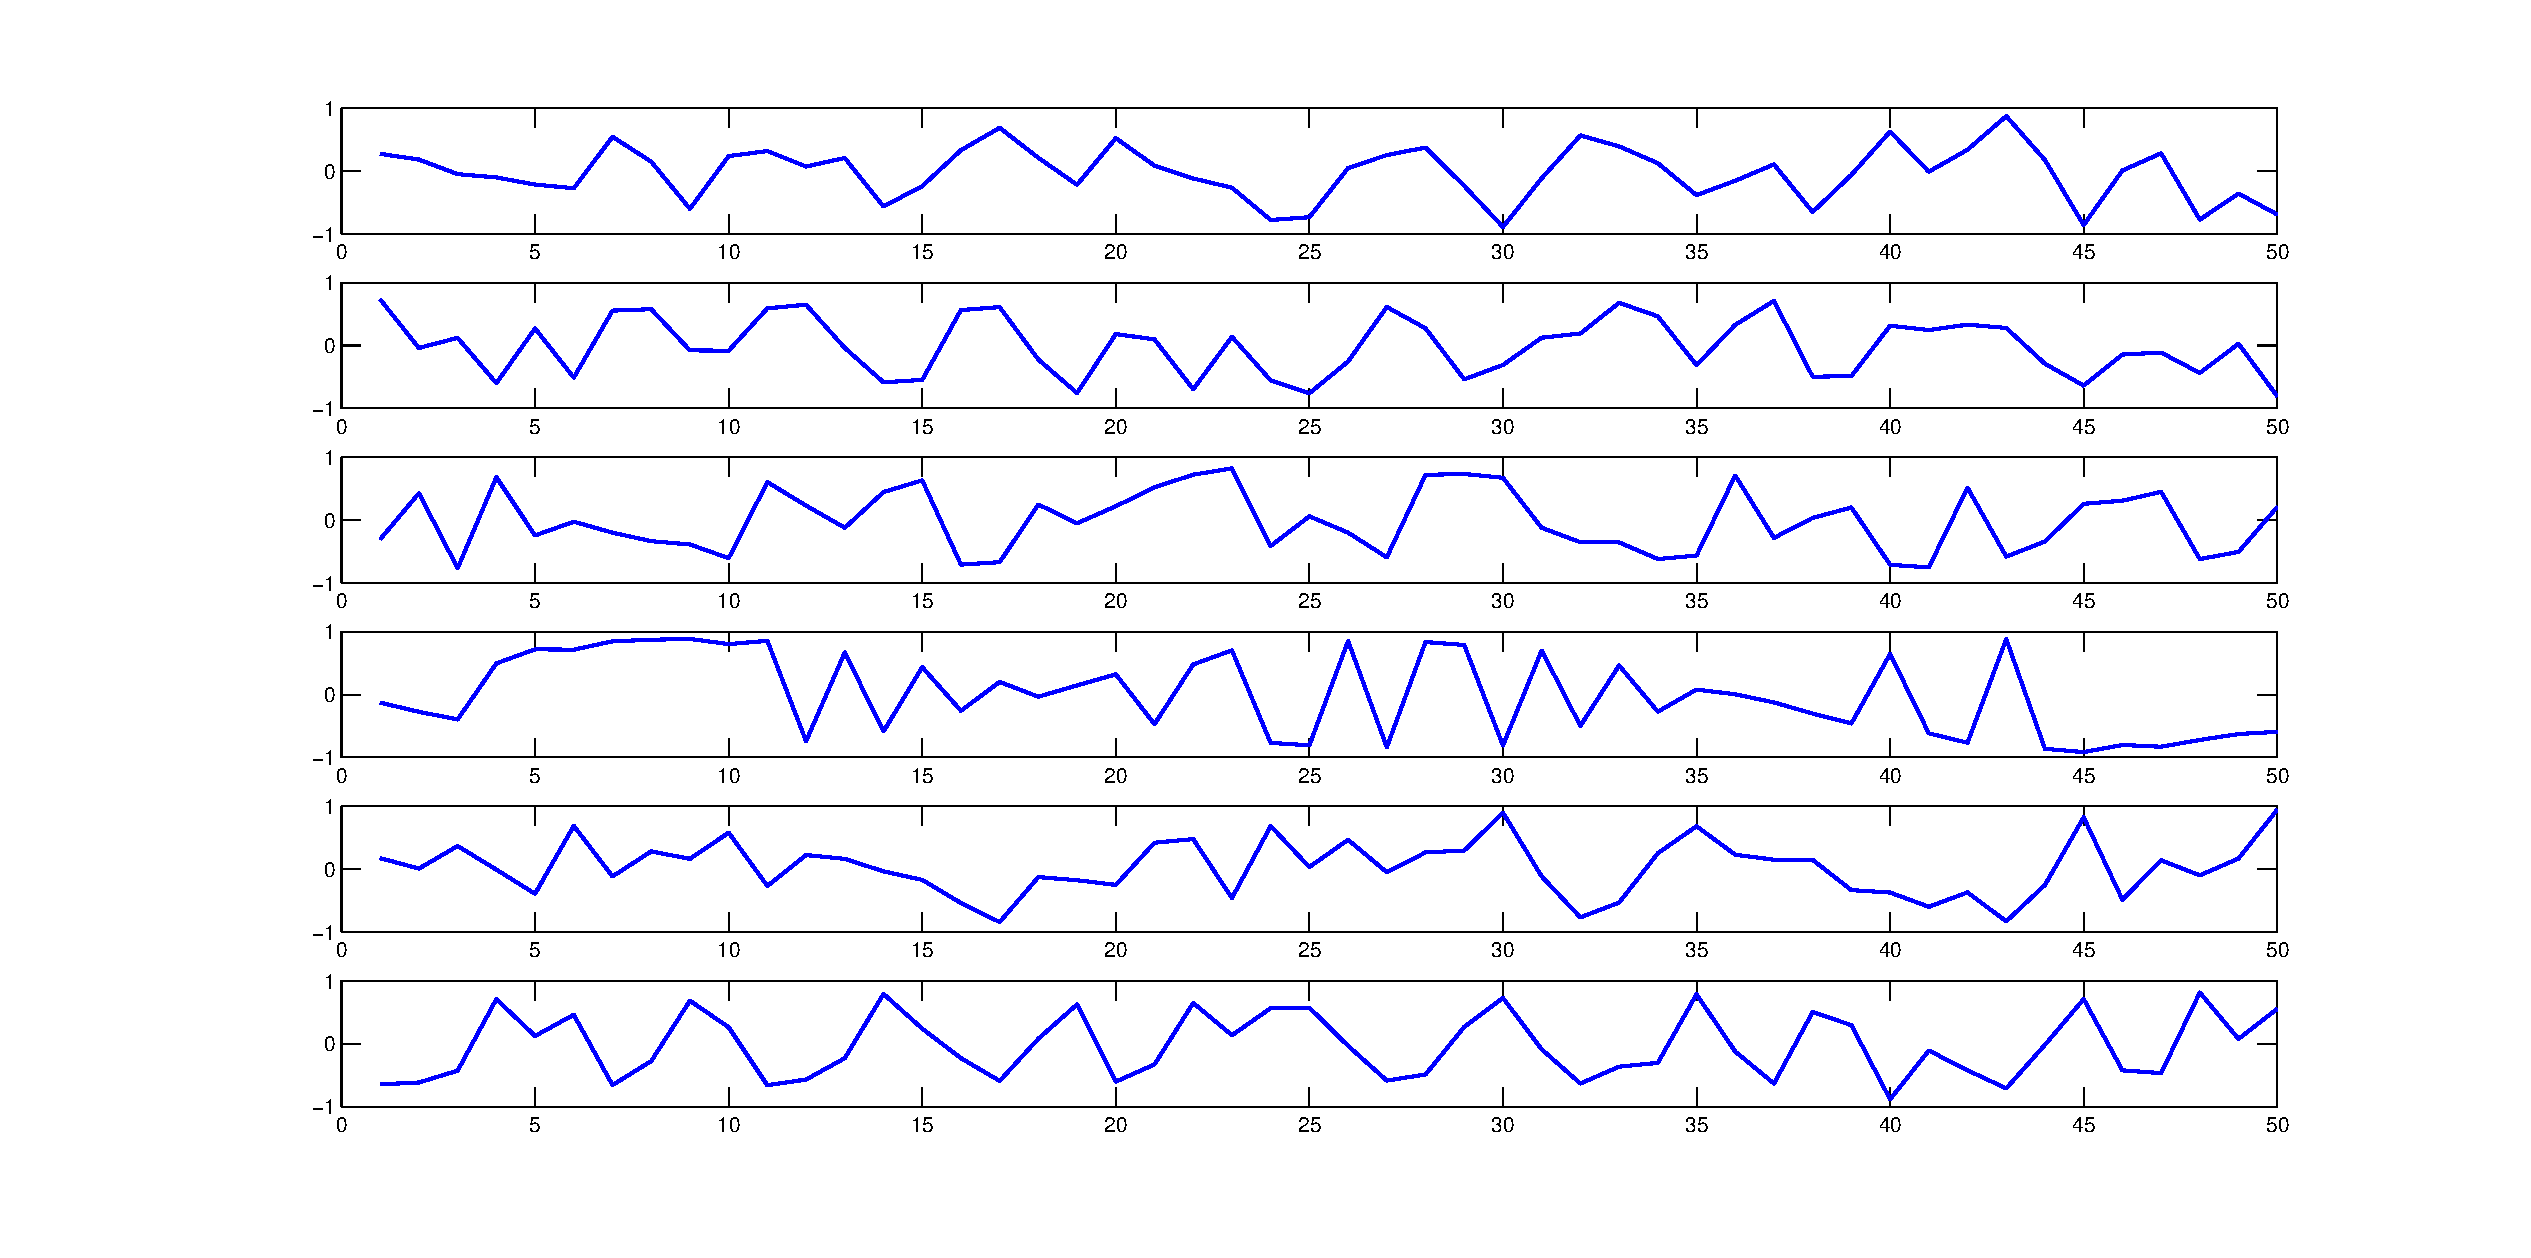
\includegraphics[width=0.5\textwidth]{Diagrams/Reconstructed-noisefree}
\ec

}

\frame{
\frametitle{Example reconstructions: Noisy case}
Noisy-free BPSK sources:
\bc
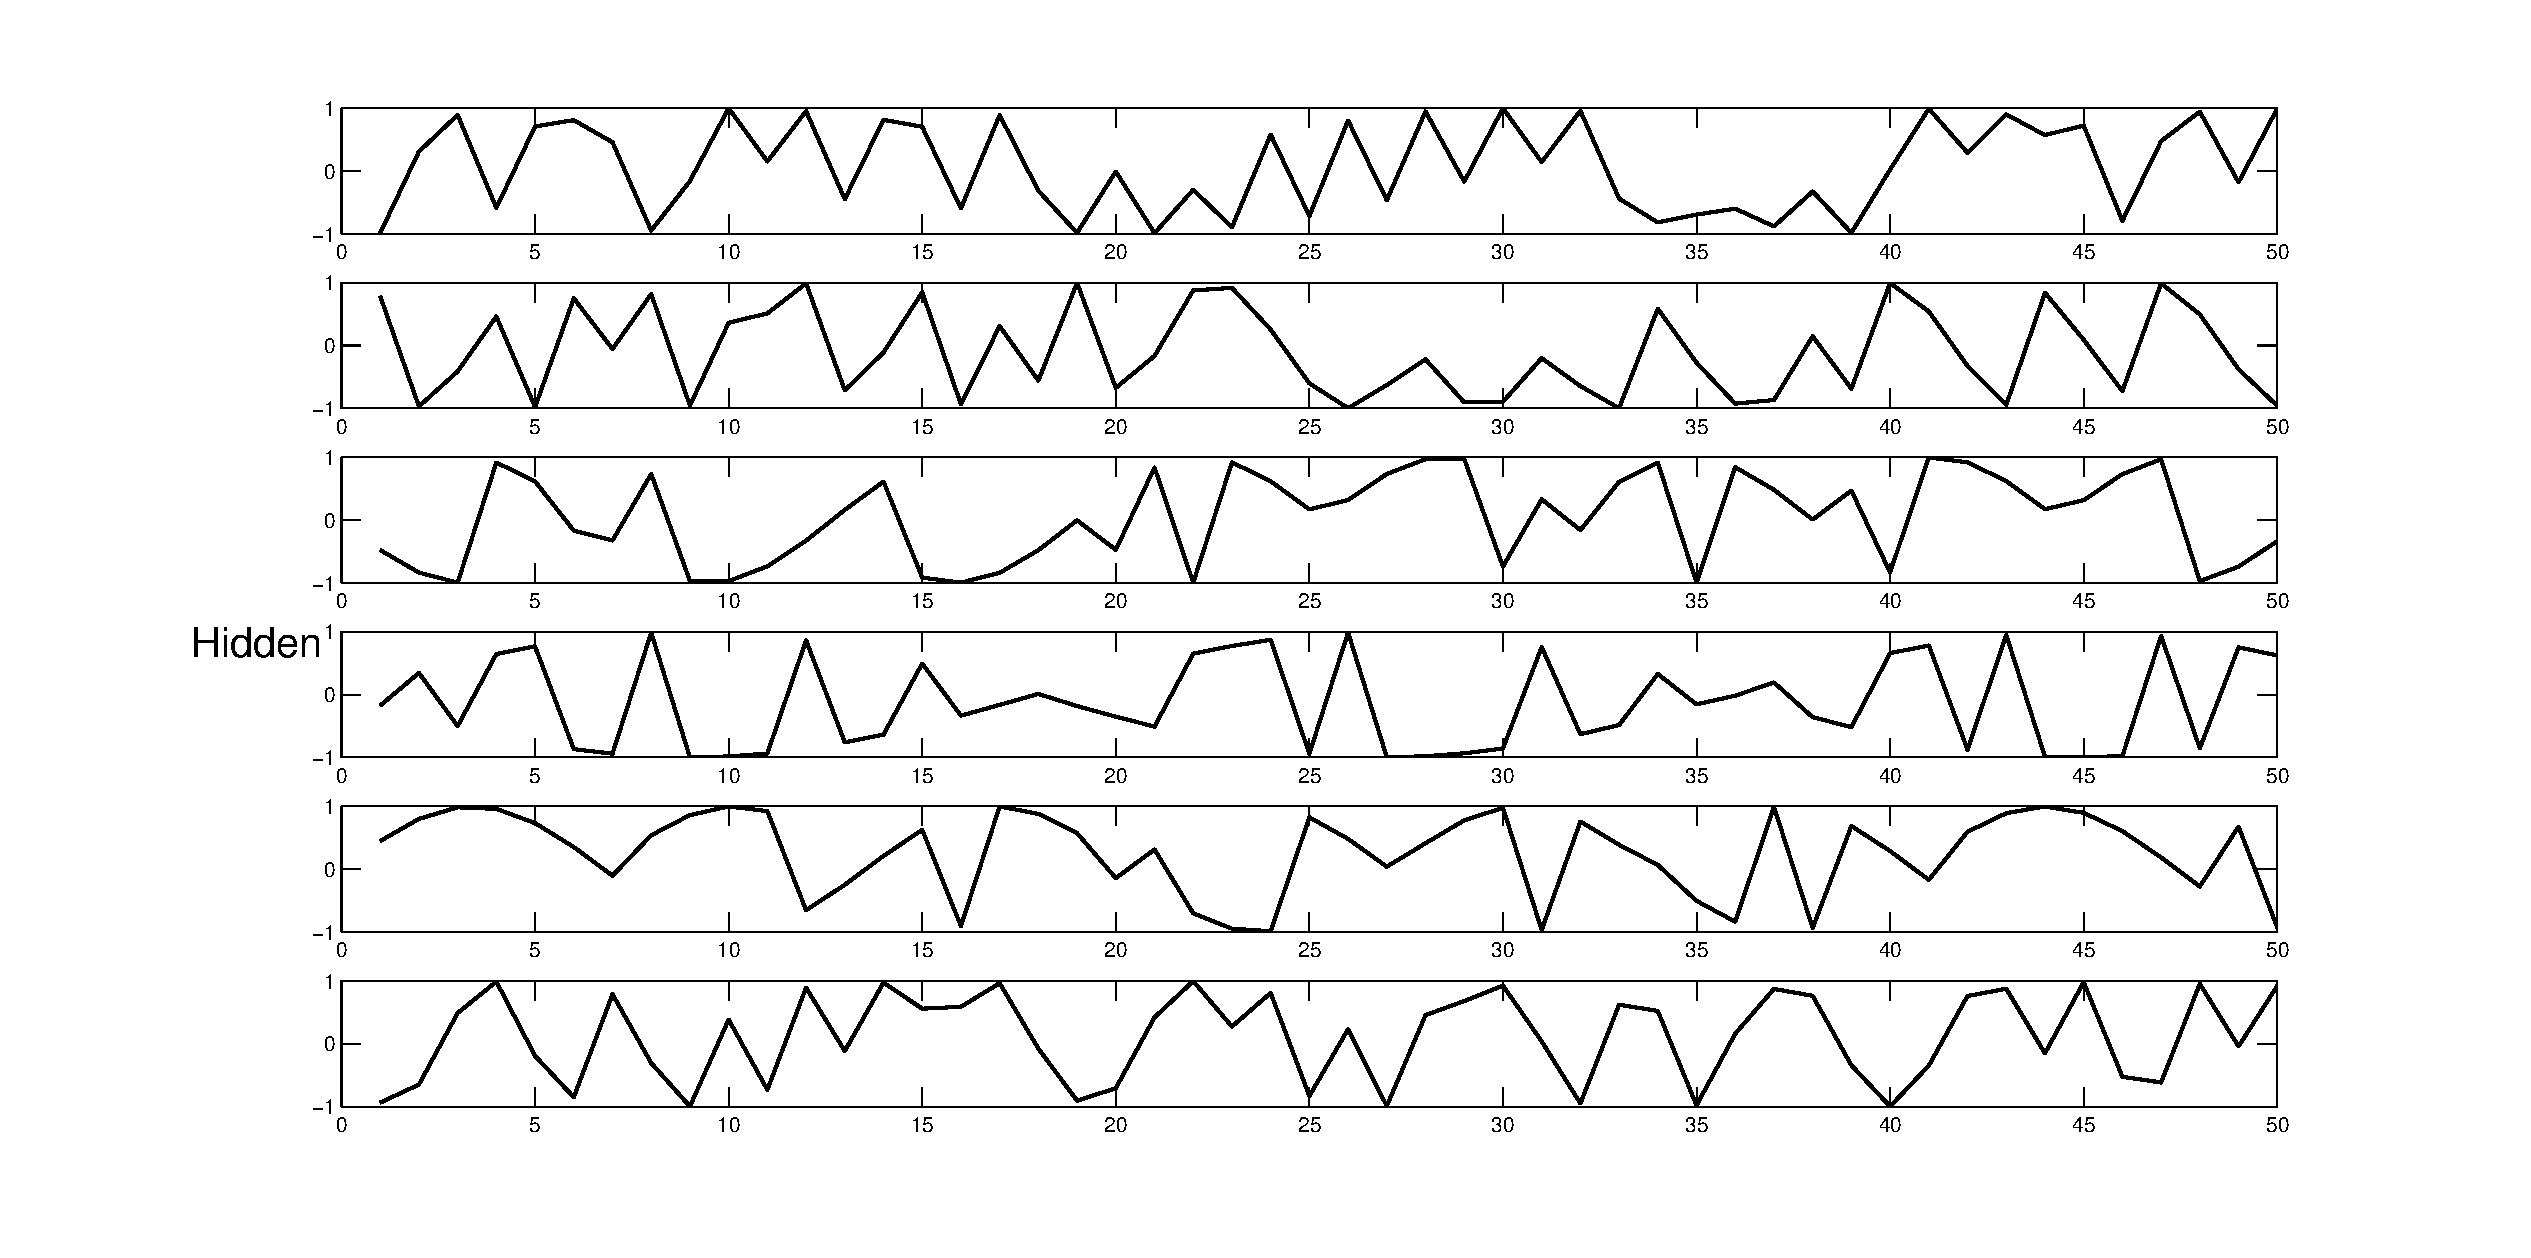
\includegraphics[width=0.5\textwidth]{Diagrams/Hidden-noisy}
\ec

Reconstruction:
\bc
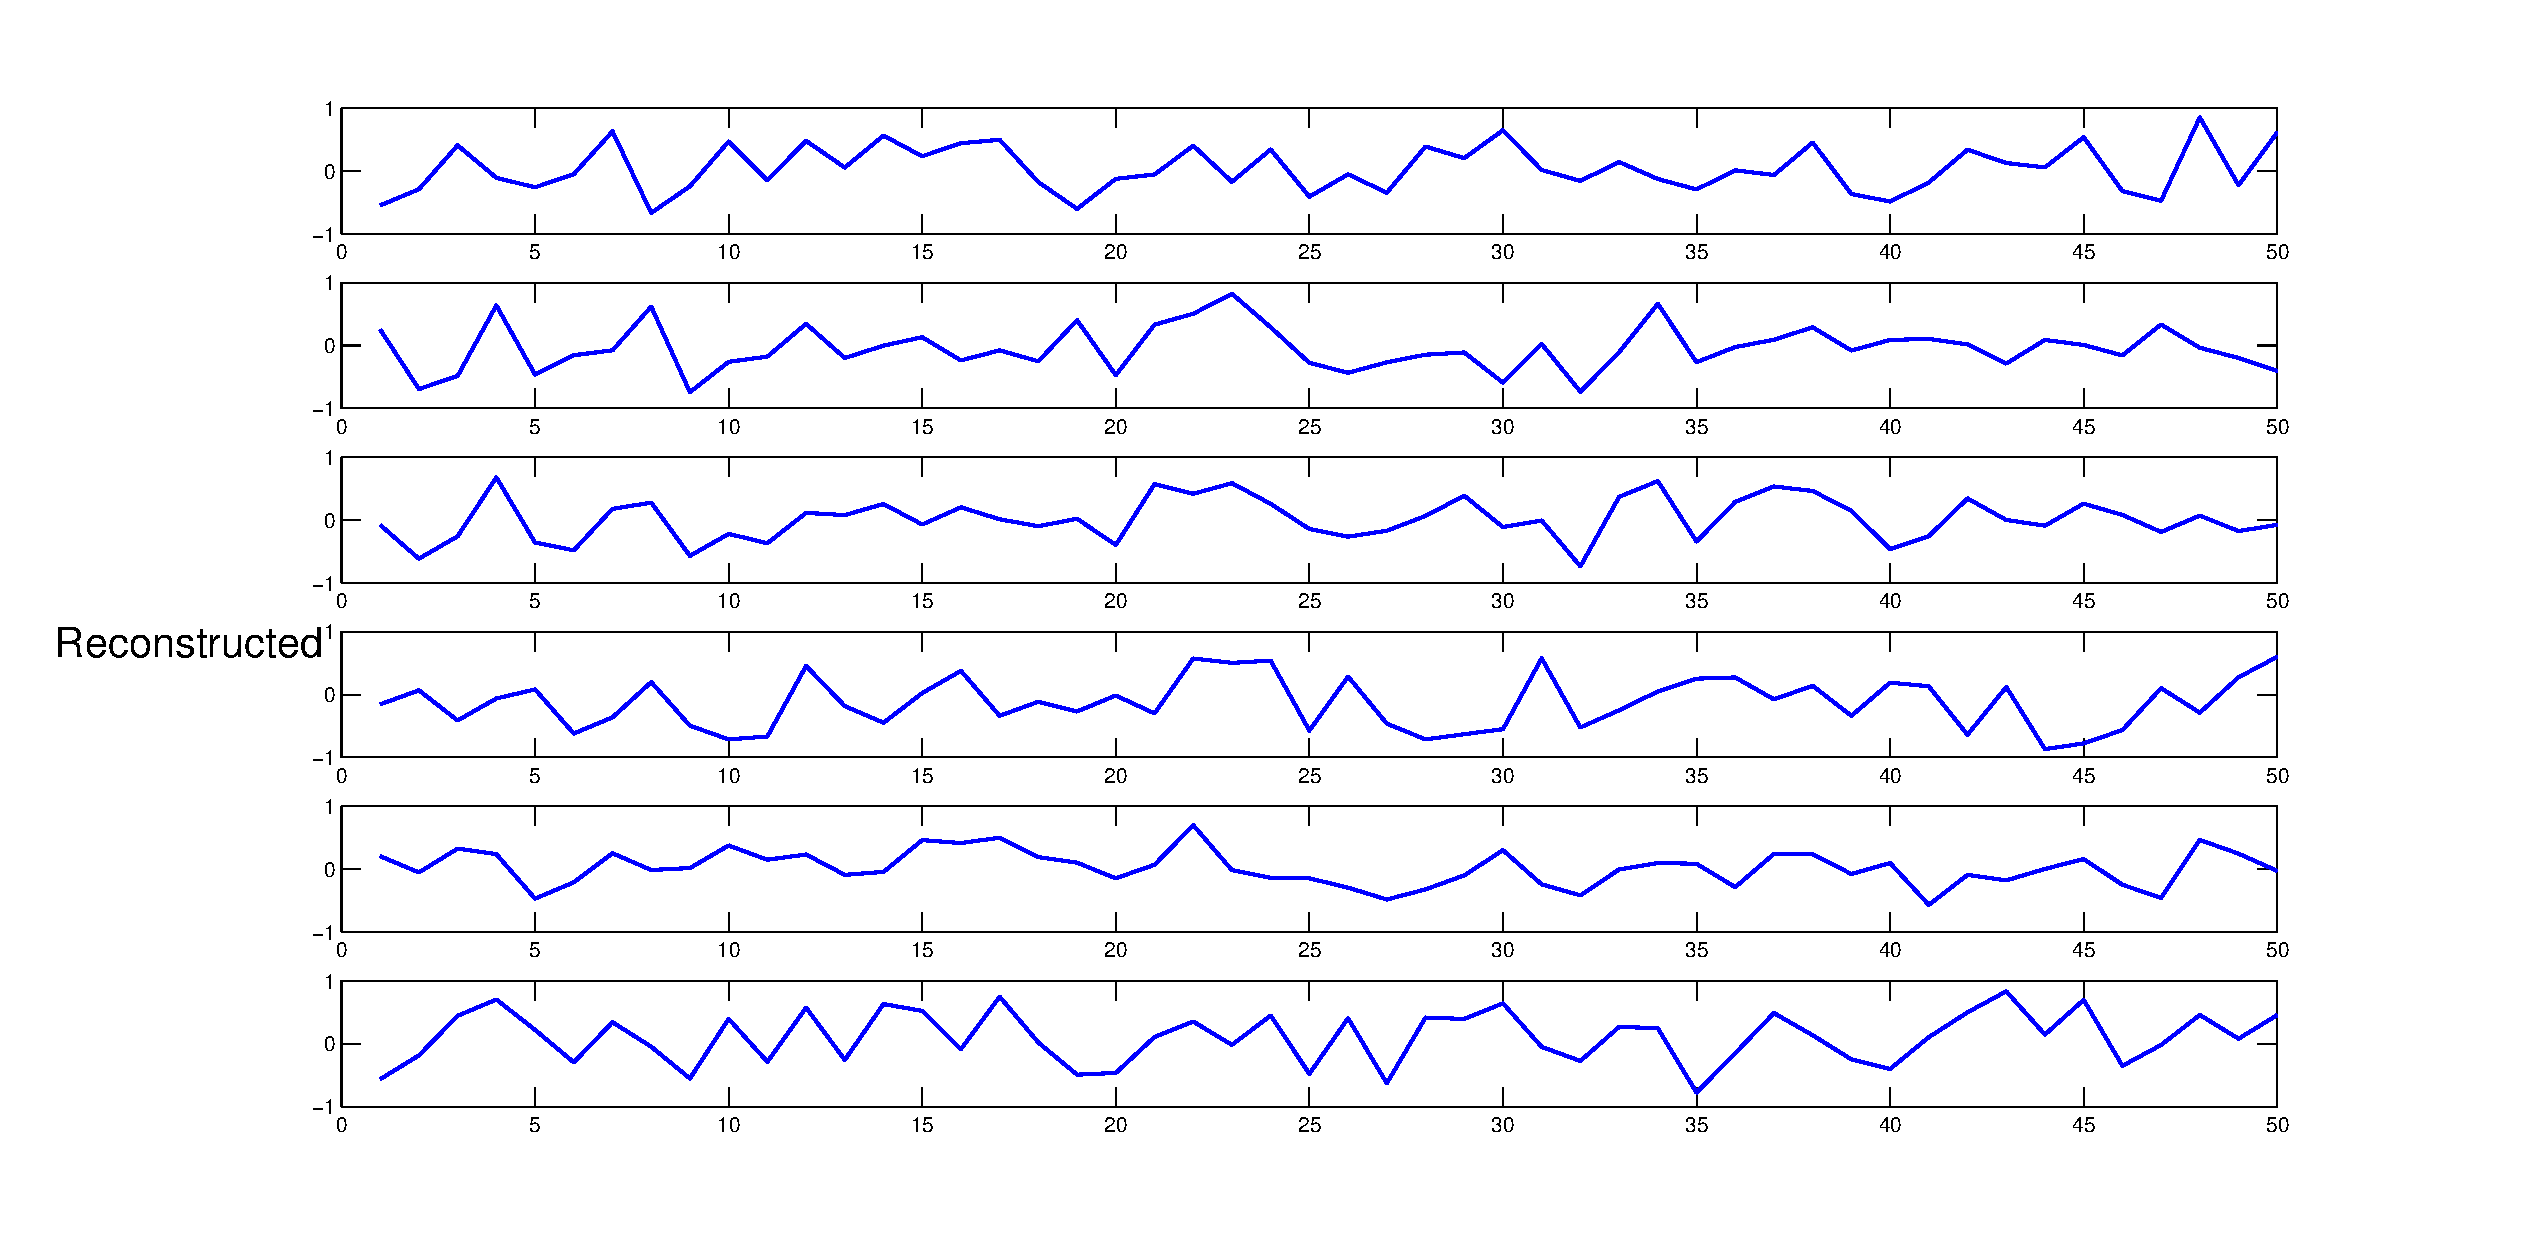
\includegraphics[width=0.5\textwidth]{Diagrams/Reconstructed-noisy}
\ec

}

\frame{
\frametitle{Turf: Noise and coherence}
\begin{columns}[t]
\column{0.5\textwidth}
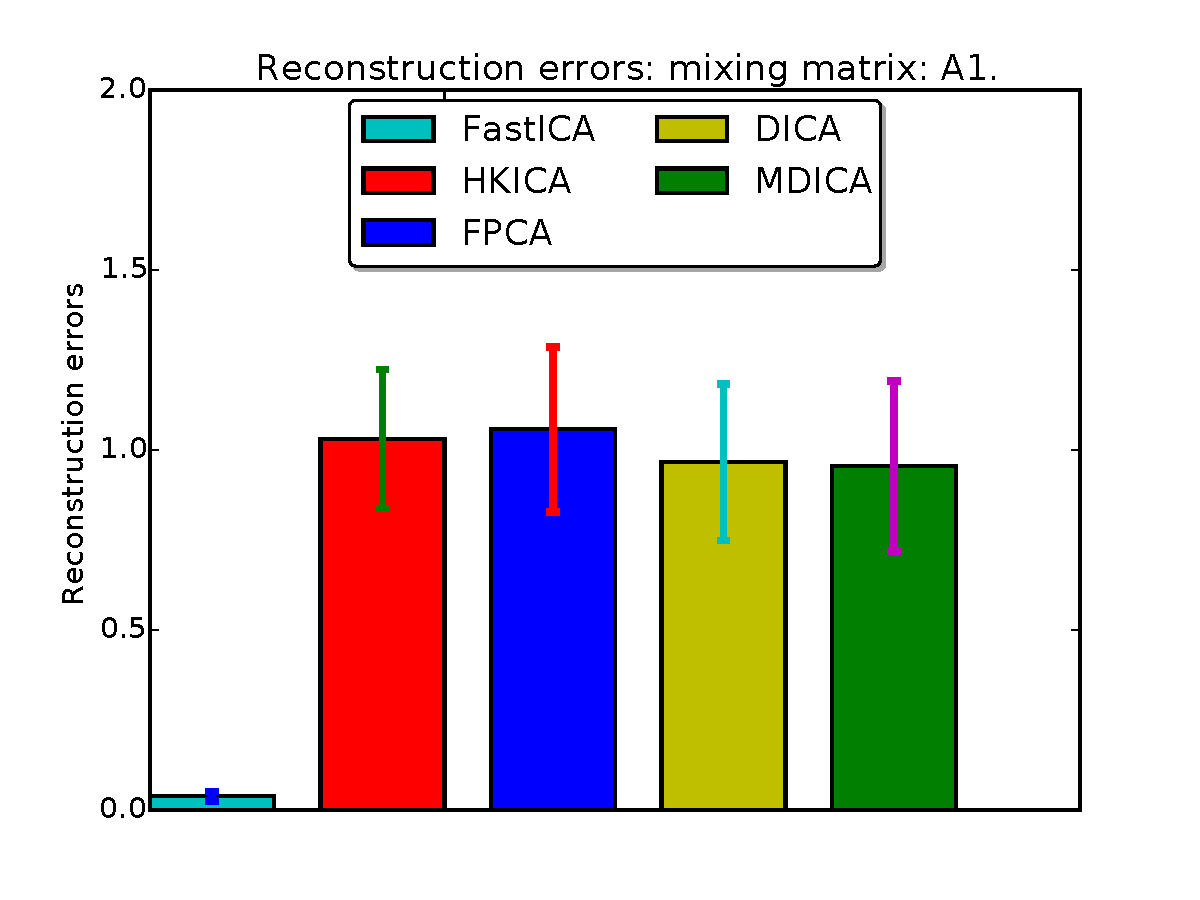
\includegraphics[width=\textwidth]{Diagrams/barchart-A1-noisefree}
\bc
Noise-free
\ec

\column{0.5\textwidth}
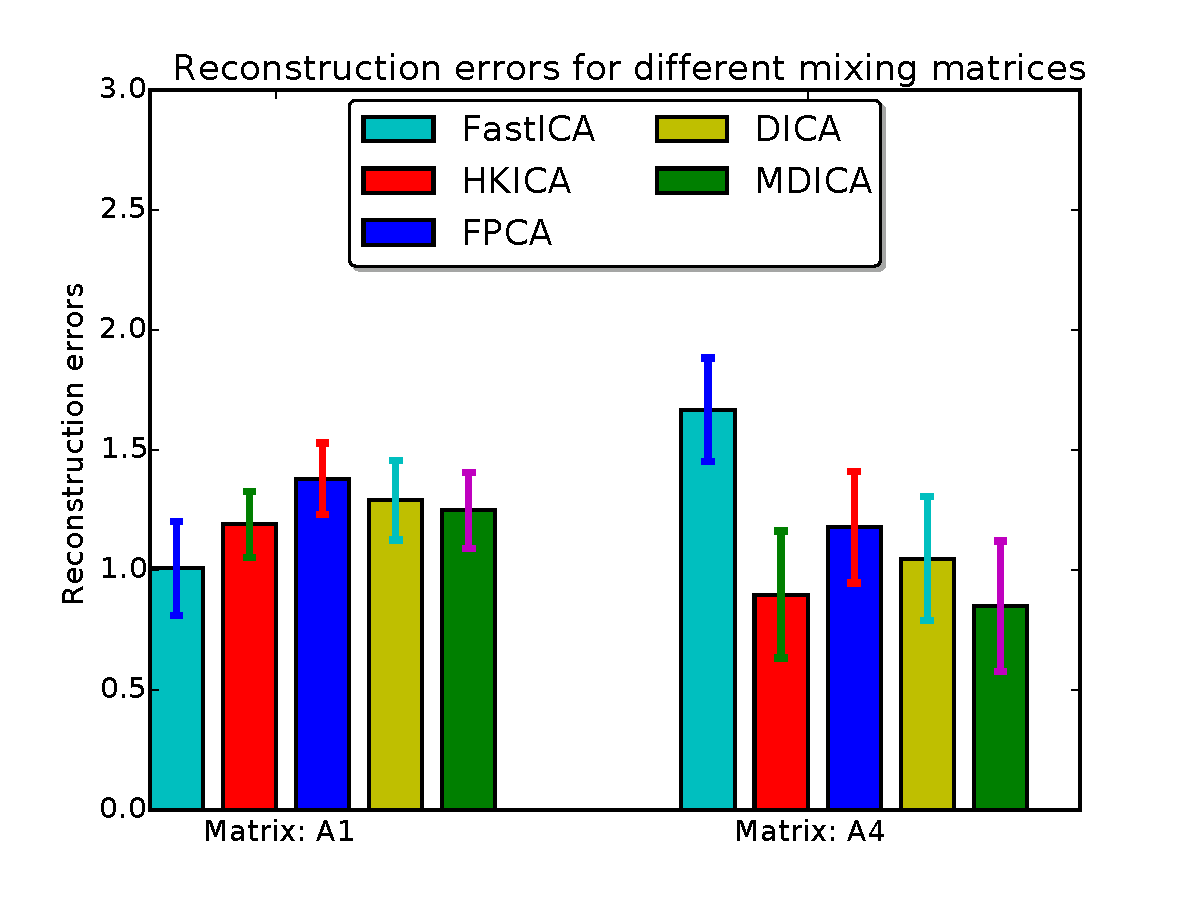
\includegraphics[width=\textwidth]{Diagrams/barchart-A1vsA4-noisy}
\bc
Noisy
\ec
\end{columns}

\bigskip

\bc
Reconstruction error of ``random'' matrix: $2.2$
\ec
}

\frame{
\frametitle{Recursive versions}
\bc
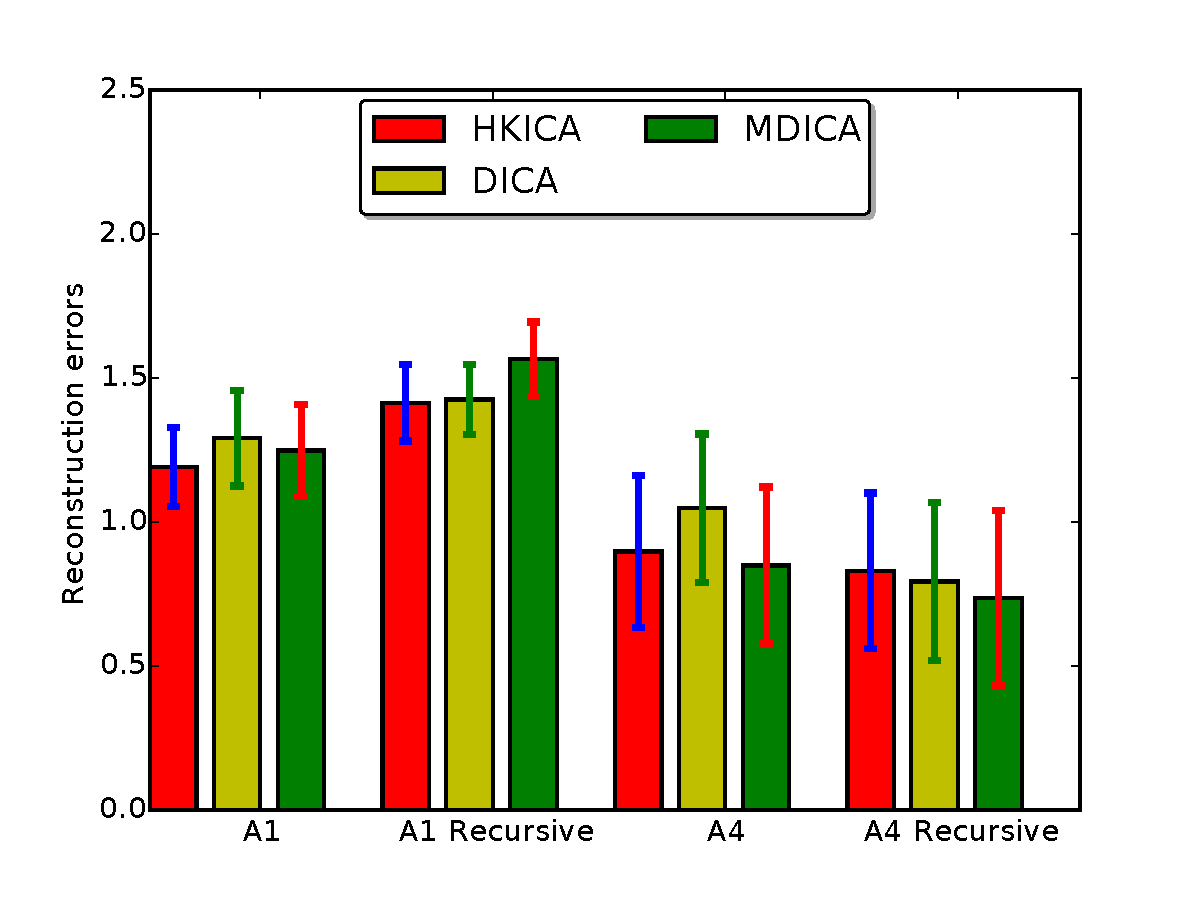
\includegraphics[width=0.5\textwidth]{Diagrams/barchart-recursive-noisy}
\ec
}


%\frame{
%\frametitle{
\if0
\vspace{-1cm}
\bi 
\item 9 different algorithms: 
	\bi
	\item<1-> HKICA (HKICA), and its recursive version (HKICA.R); 
	\item<1-> DICA  (DICA), and its recursive version (DICA.R); 
	\item<1-> A heuristic modification of  DICA  (MDICA), and its recursive version (MDICA.R);
	\item<1-> The default FastICA algorithm \citep{szabo12separation} (FICA);
	\item<1-> The recursive Fourier PCA \citep{vempala2014max}(FPCA);
	\item<1-> Random guessing (Random).
	\ei
\item 5 types of mixing matrices:
	\bi 
	\item<2-> $A = R$ is an orthonormal matrix;
	\item<2-> $A(A_1) = P$; 
	\item<2-> $A(A_2) = v_b\times\boldsymbol{1}' + 0.3\times P$;
	\item<2-> $A(A_3) = v_b\times\boldsymbol{1}' + 0.05\times P$;
	\item<2-> $A(A_4) = v_b\times\boldsymbol{1}' + 0.005\times P$  
	\item The vector $v_b$ and the matrix $P$ are both generated from standard normal distribution, and then normalized.
	\ei
\ei
}
\fi

\if0
\frame{ \frametitle{Setting}
\bi
\item 6-dimensional BPSK signals with different periods;
\item $x = As + c\eps$ for different noise ratio coefficients $c$;
\item $T = 20000$ observations;
\item Results are evaluated on a 150 repetitions. For each repetition, we try 3 times and report the best.
\ei
}

{\nologo
\frame{ \frametitle{Simulation resutls}
\begin{multicols}{3}
	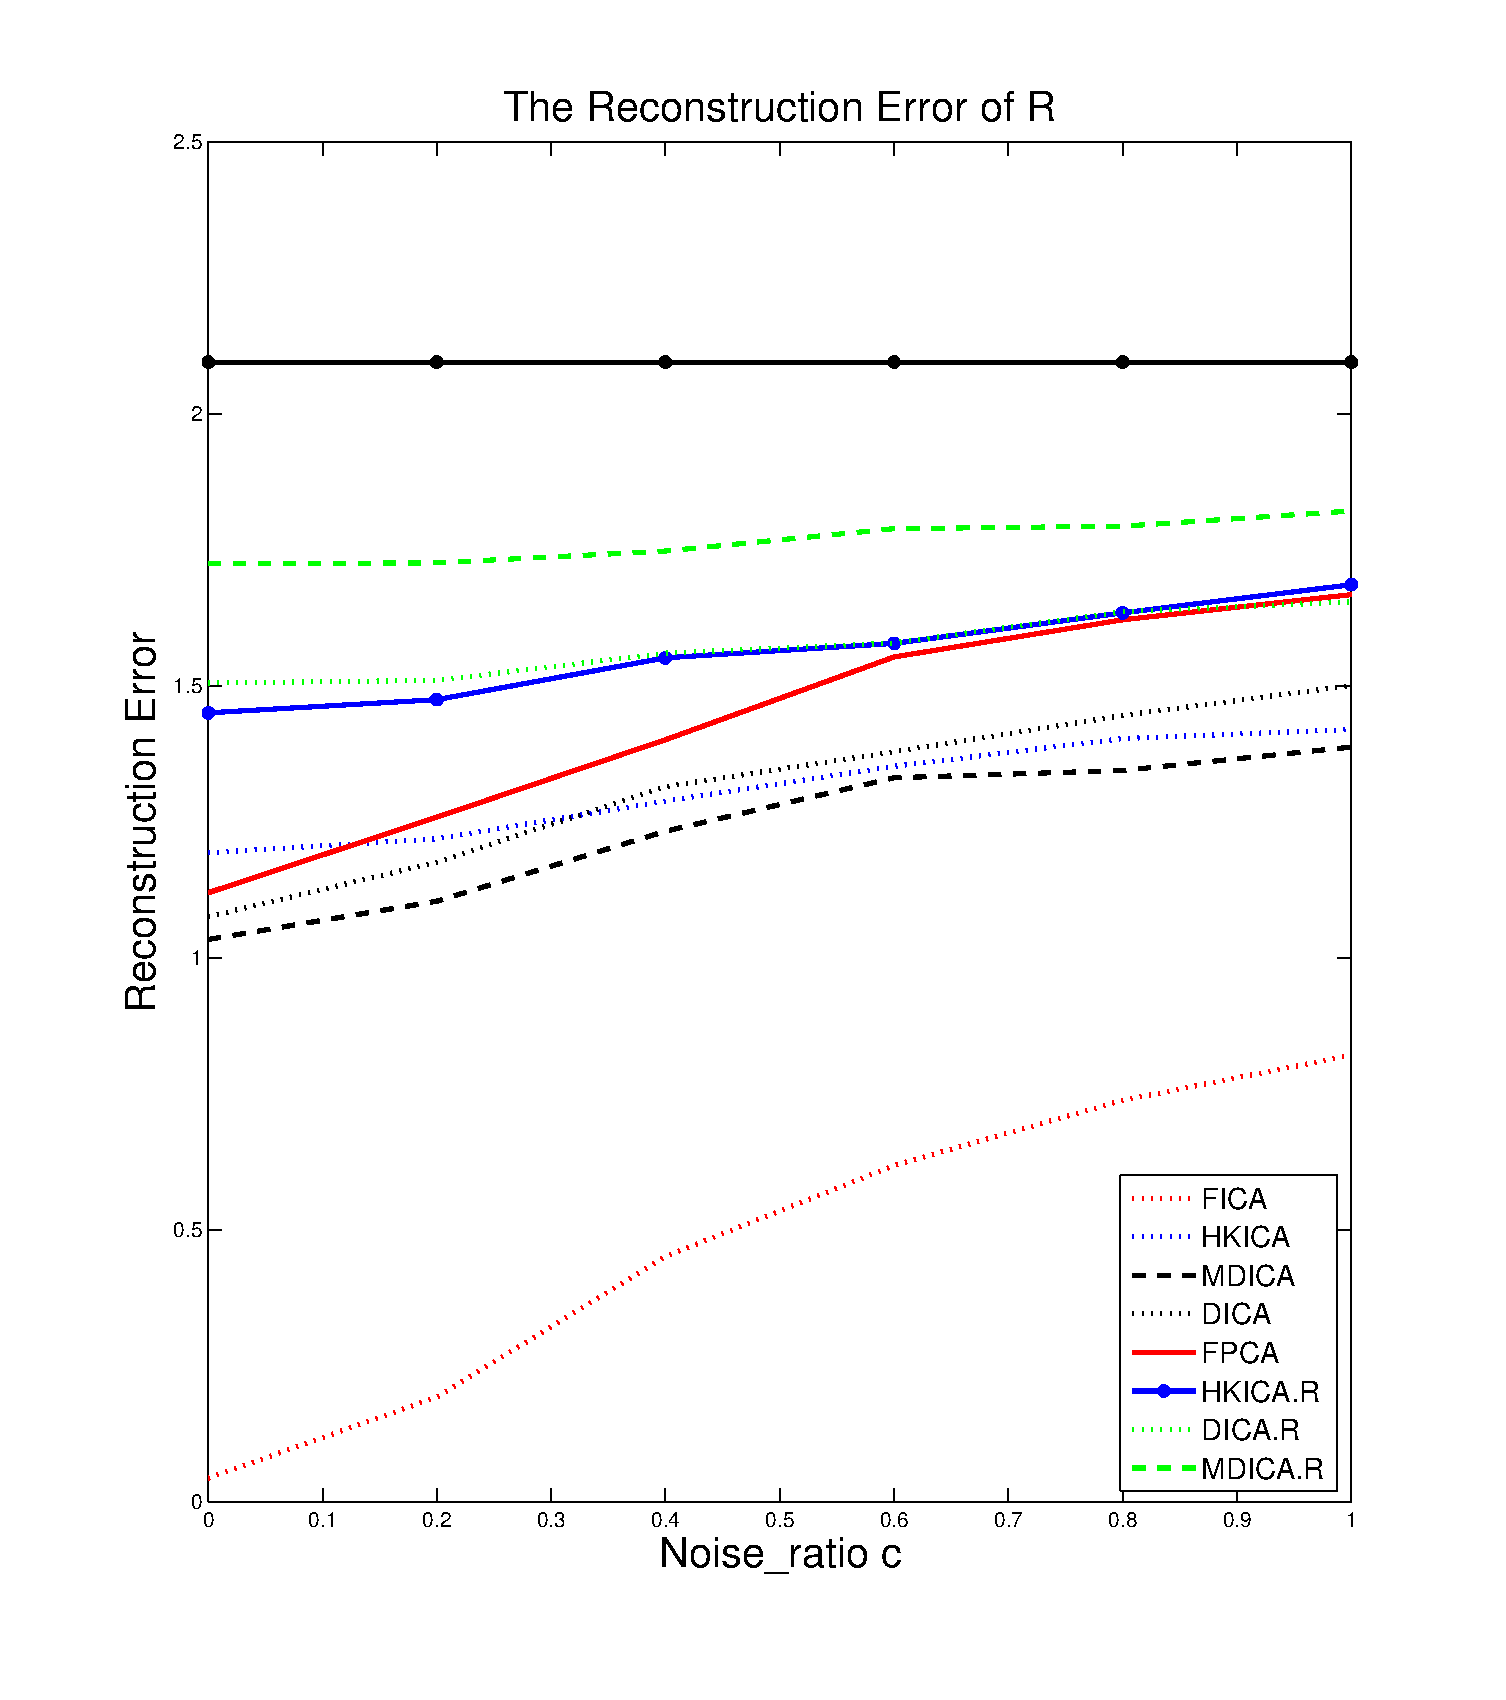
\includegraphics[height = 0.42\textheight]{errorR}\\
	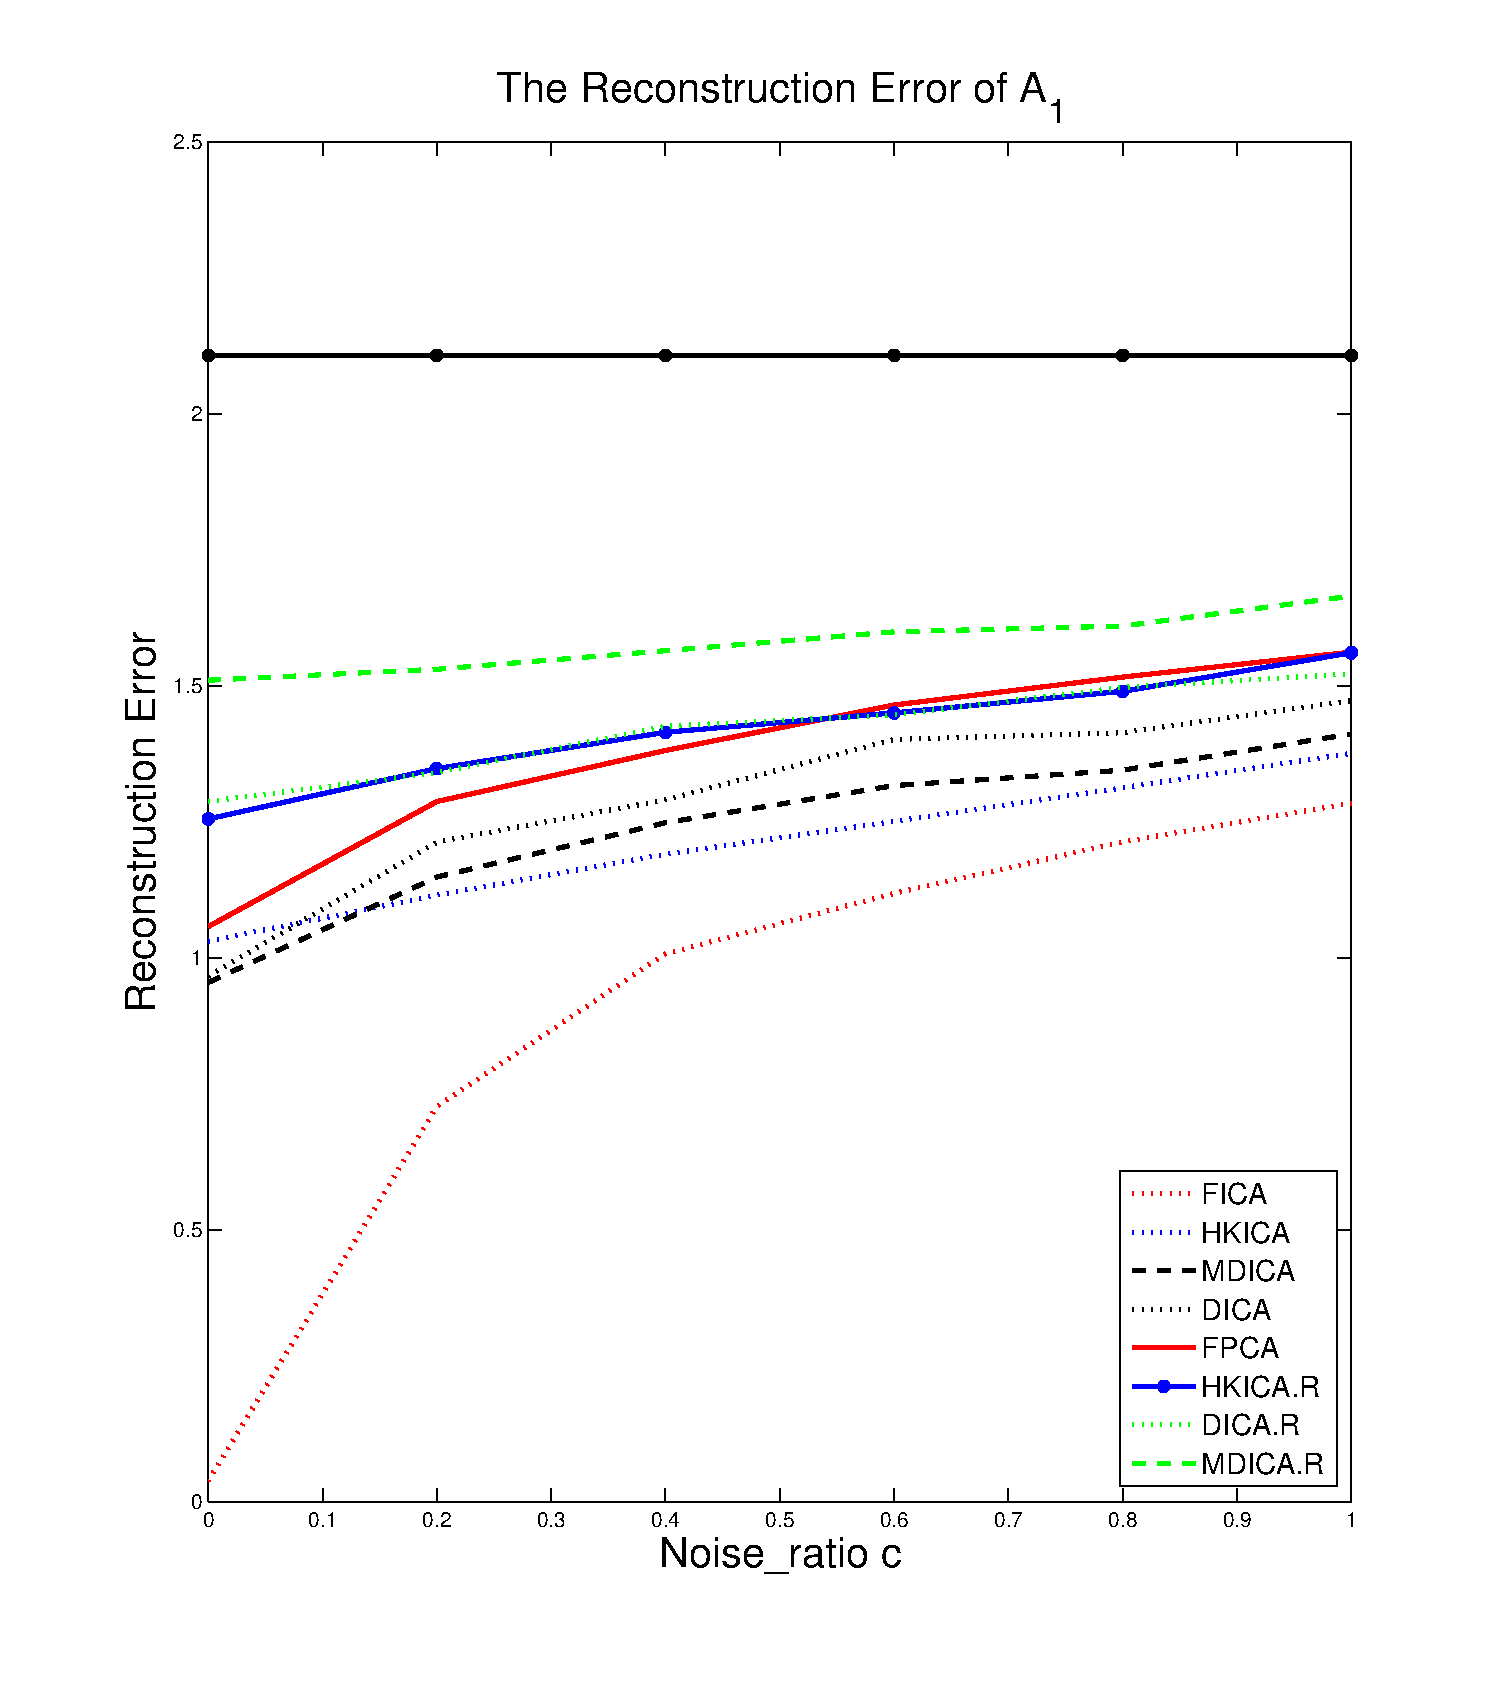
\includegraphics[height = 0.42\textheight]{error1}
	\newpage
	\topskip0pt
	\vspace*{\fill}
	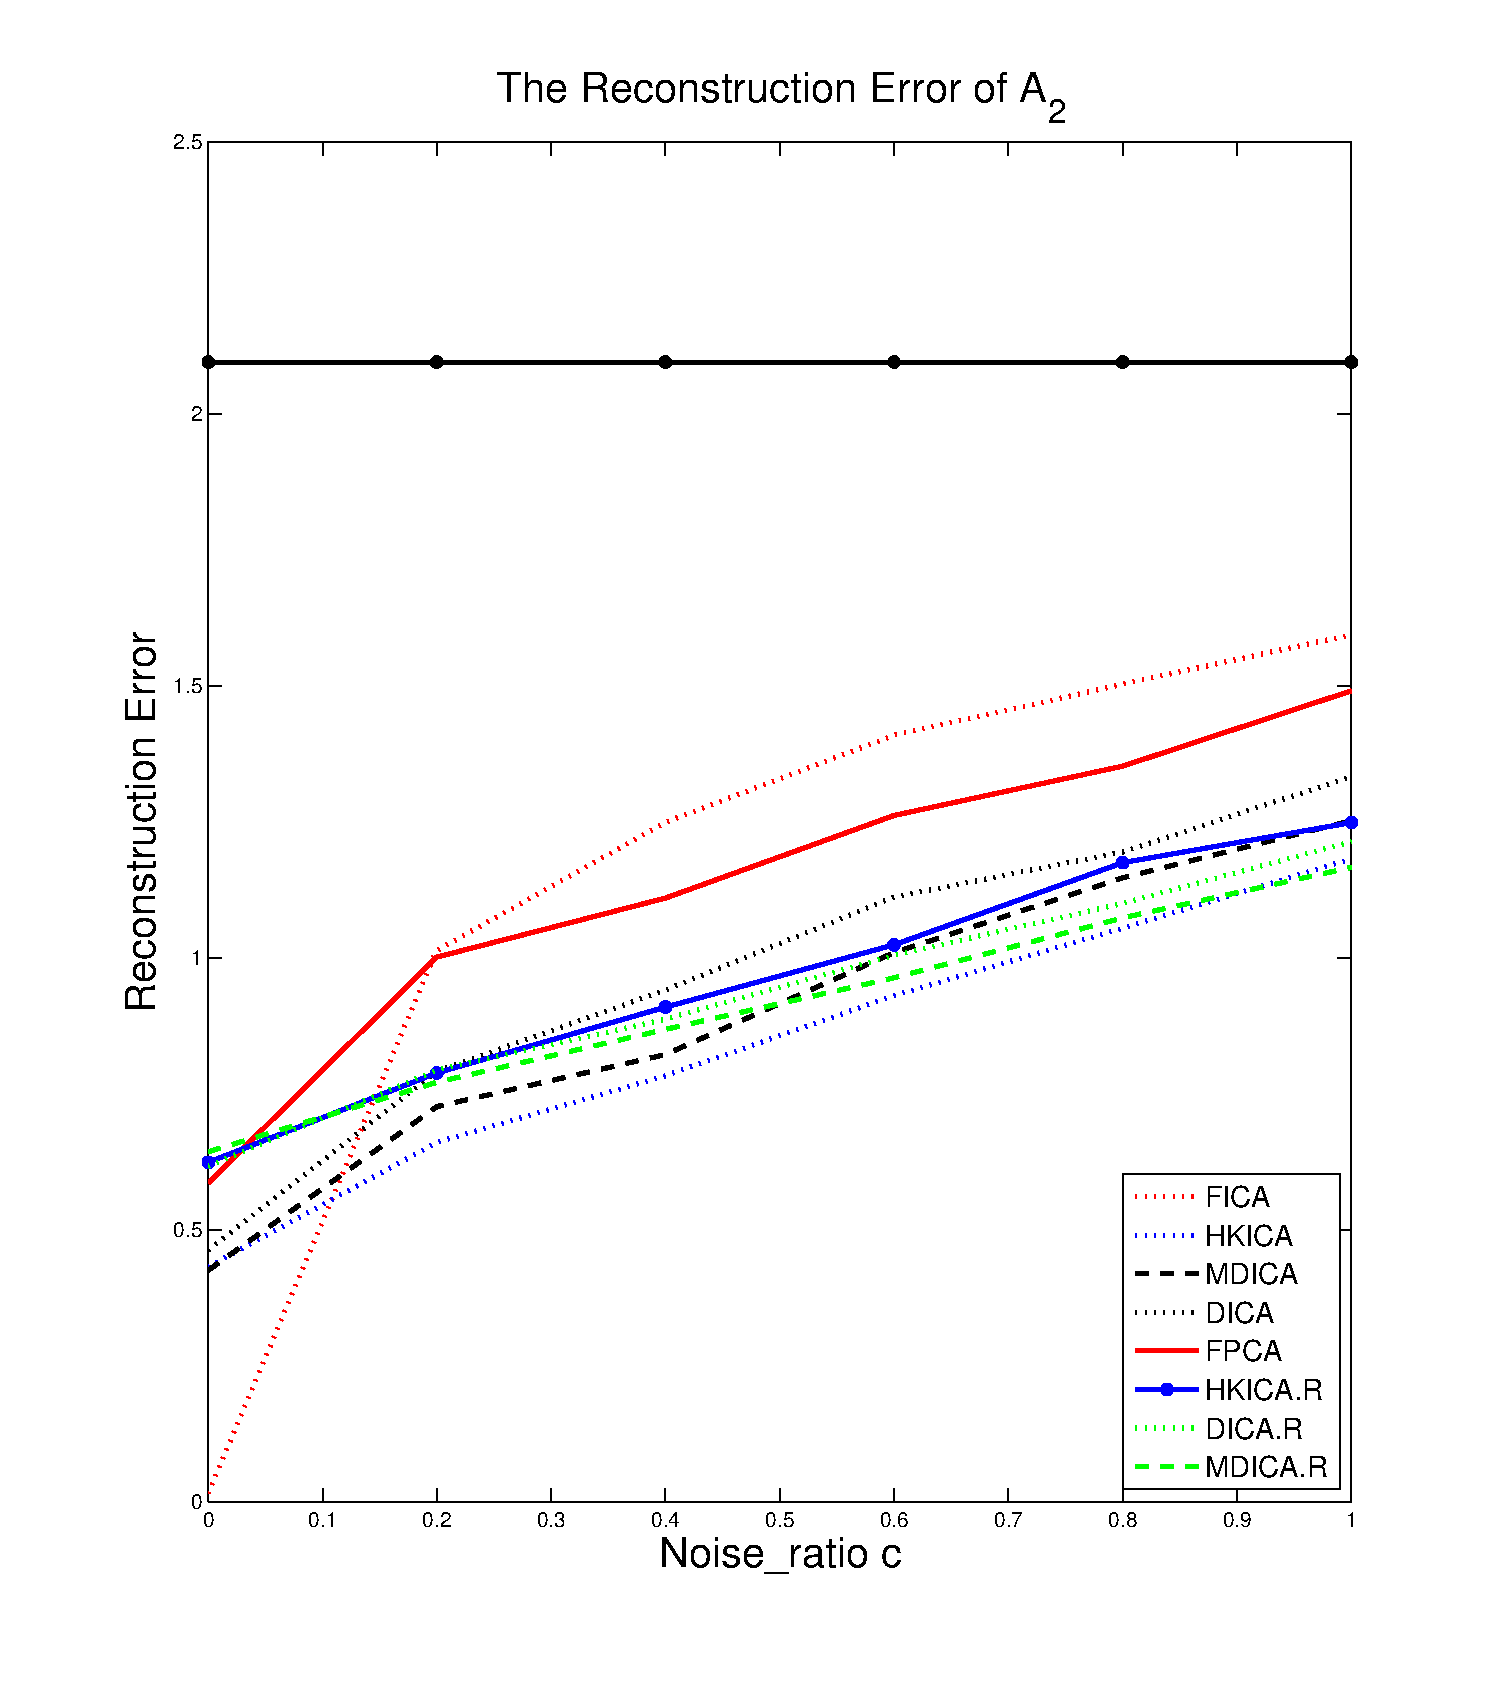
\includegraphics[height = 0.42\textheight]{error2}
	\vspace*{\fill}
	\newpage
	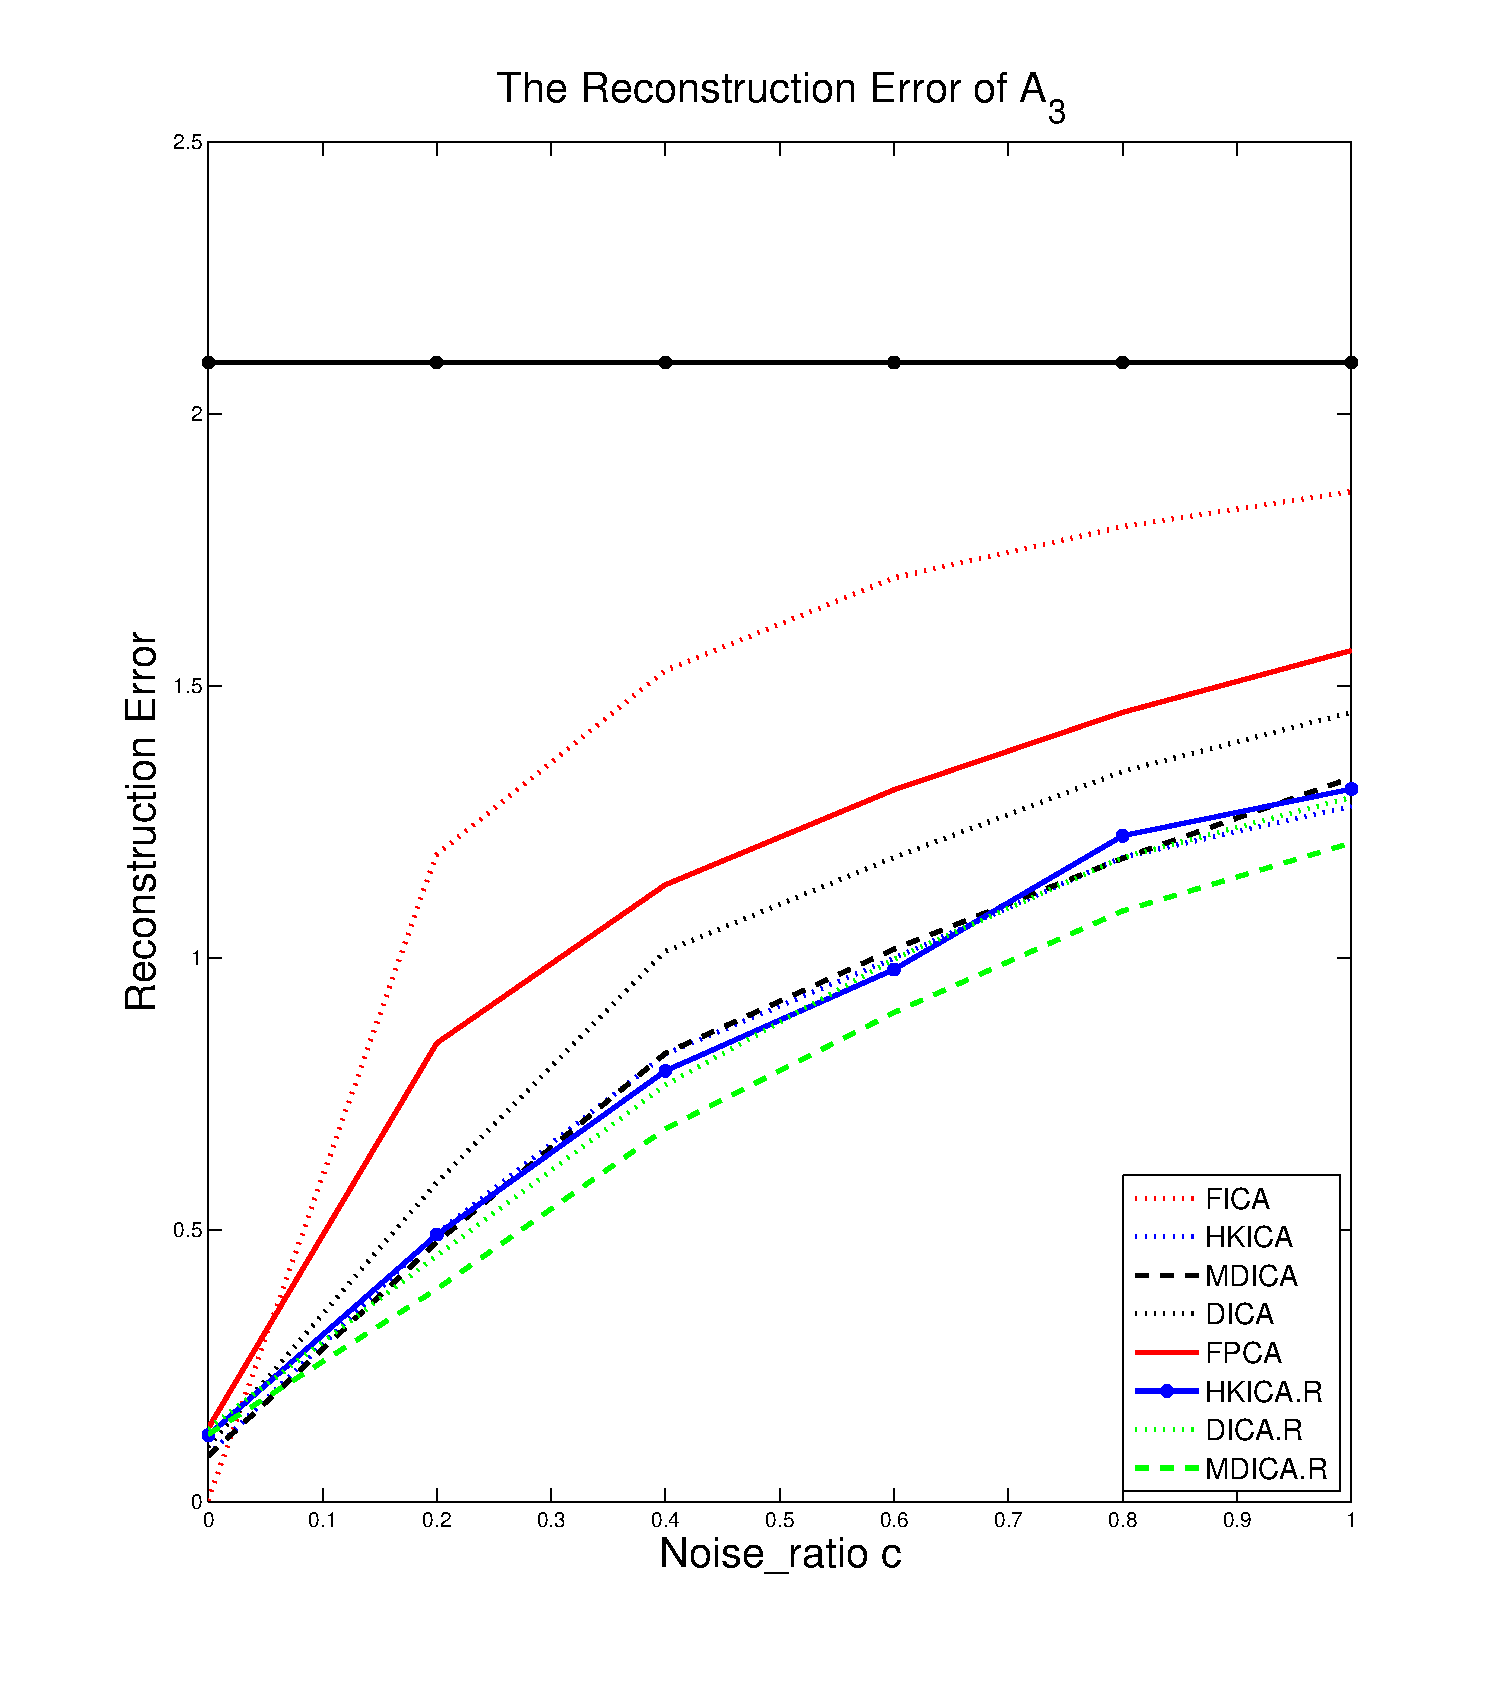
\includegraphics[height = 0.42\textheight]{error3}\\
	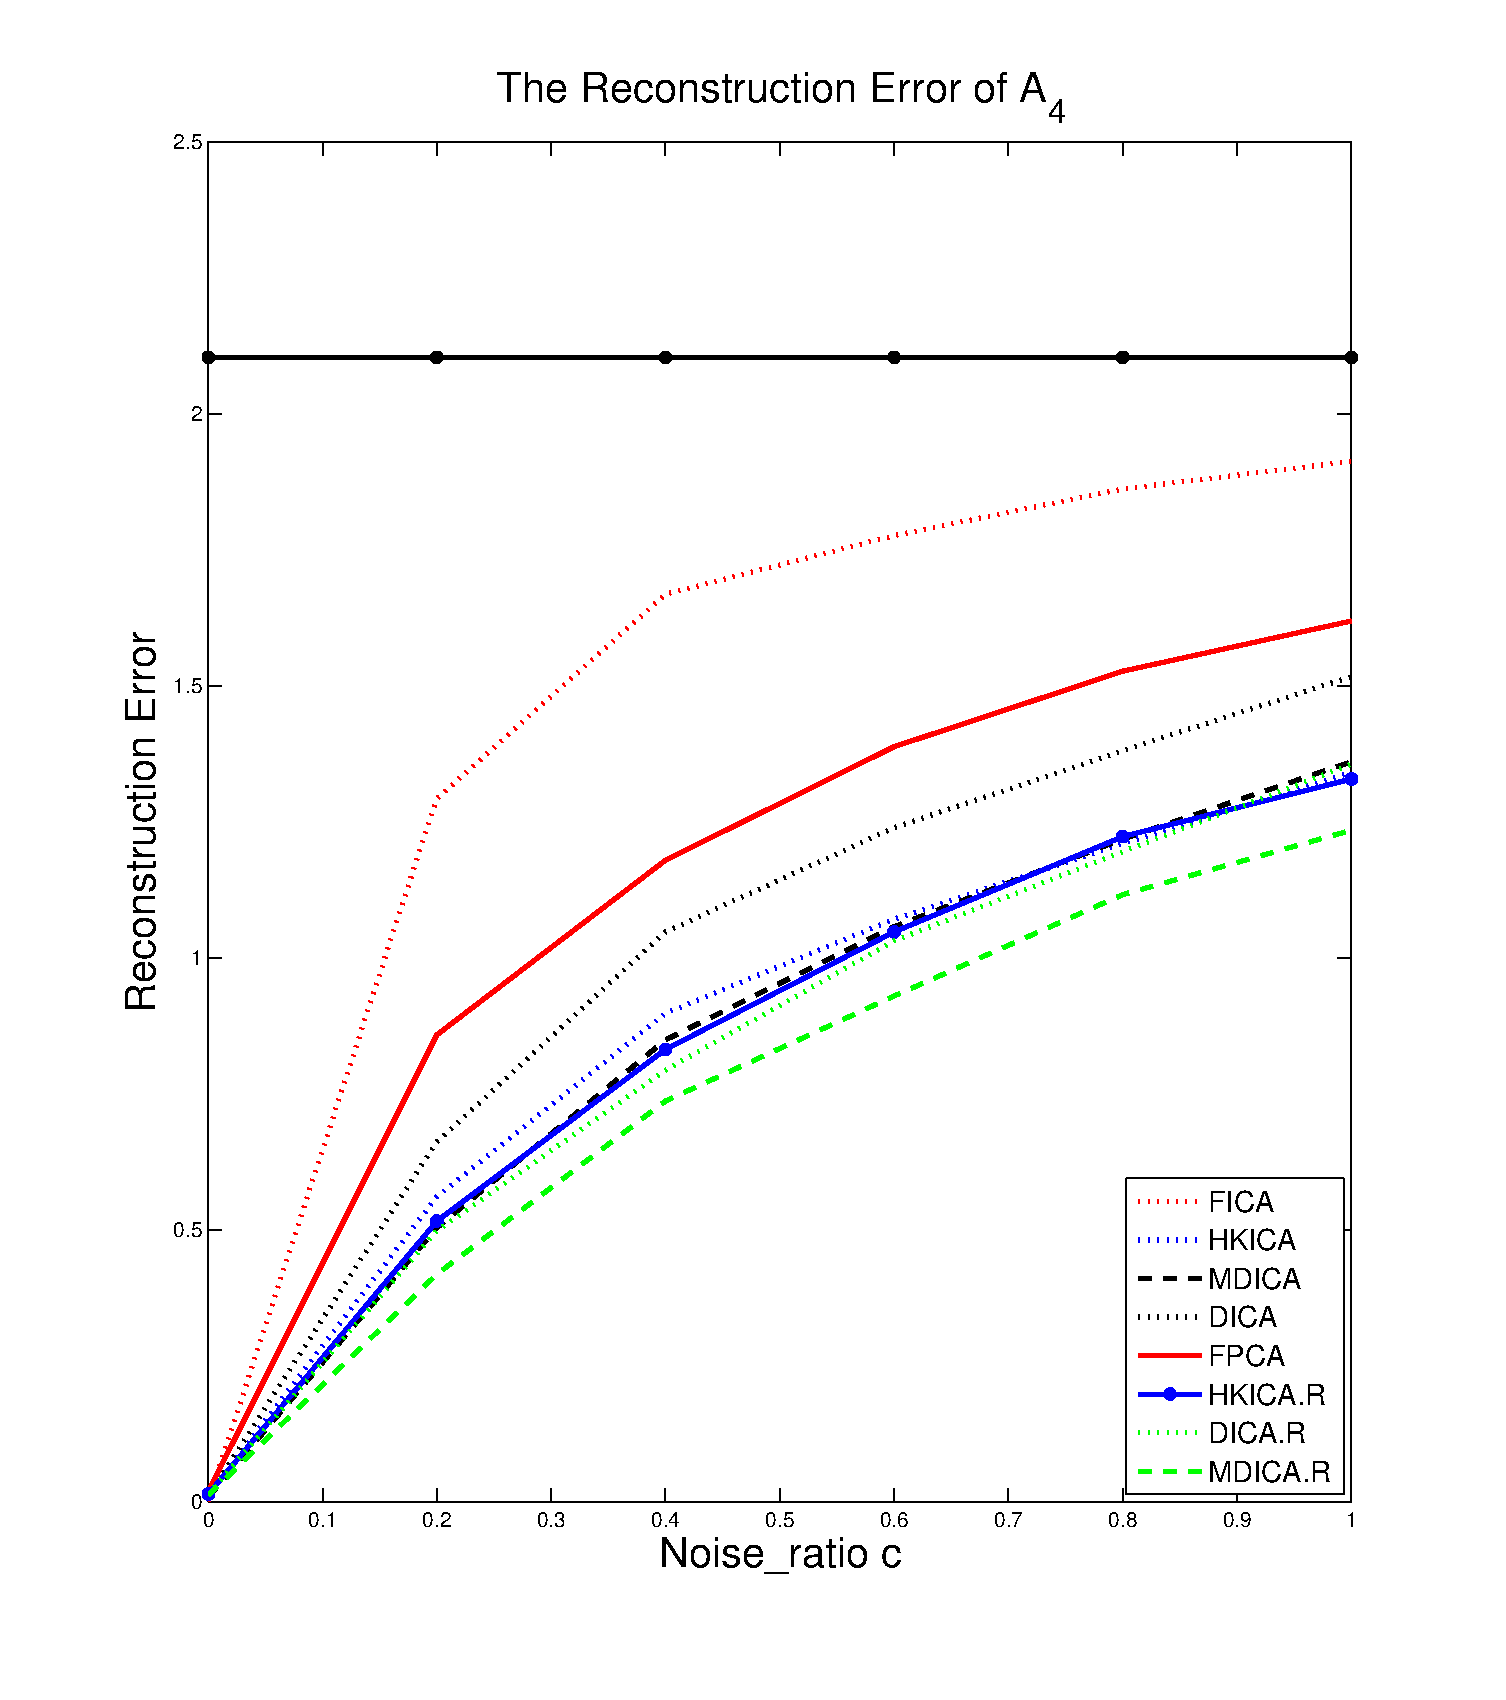
\includegraphics[height = 0.42\textheight]{error4}
\end{multicols}
}
}
\fi

\section{Conclusions}
\begin{frame}{Outline}
\tableofcontents[currentsection]
\end{frame}

\frame{\frametitle{Conclusions}

\bi
\item[\ds] Independent Component Analysis without probabilities! 
\item[\ds] Deterministic analysis: Cleaner, more general, should do it more often! Limits?
\item[\ds] New method: DICA. Universal, strong guarantees.
\item[\ds] In practice, moment-methods are indeed more robust to noise.
\item[\ds] HKICA is great! Why? MDICA is also good. Why?
\item[\ds] ``Recursive versions'': No significant advantage was found (limited study?).
\ei

\uncover<+->{
\centering \LARGE \textcolor{blue}{Questions?}
}
}

\if0
\frame{ \frametitle{Simulation results} 
\bi
	\item Moment methods are more robust to high-coherence mixing matrices and Gaussian noise;
	\item We don't really observe improvement of DICA from HKICA in the experiments: estimation error explodes;
	\item MDICA works best, but this method only has weak theoretical guarantee;
	\item The recursive idea seems not always helpful: theoretically it only helps in the eigen-decomposition step.
\ei
} 
\fi

\frame{ \frametitle{References}
\tiny
\bibliographystyle{abbrvnat}
\bibliography{DICA}
}

\if0

\frame{ \frametitle{\,}
\begin{center}
{\huge Thank you !}
\par\end{center}{\huge \par}
\begin{center}
{\huge Questions?}
\par\end{center}{\huge \par}
} 
\fi
\end{document}
